\documentclass[titlepage, a4paper, 11pt]{article}


\usepackage[english]{babel}

\usepackage[a4paper, left=1in,right=1in,top=1in,bottom=1in,]{geometry}

% Useful packages
\usepackage{amsmath}
\usepackage{subcaption}
\usepackage{float}
\usepackage{biblatex}
\addbibresource{sample.bib}
\usepackage{graphicx}
\graphicspath{ {./images/} }
\usepackage[]{hyperref}



\usepackage{caption}
\captionsetup{font=small}

\begin{document}
\begin{titlepage}
	\begin{center}
		\vspace*{1cm}
        \hline
        \vspace{0.4cm}
		\textbf{\Huge Fluid Mechanics Project Report}
		\vspace{0.4cm}
		\hline

		\vspace{2cm}
		\textbf{\huge{Fluid Flow Through an Expansion }}

		\vspace{5cm}
		
		
        
\includegraphics[width=0.7\textwidth]{images/task1/Koc_Logo.png}
        
        
        \vfill
        
		\Large{Deniz Erdogan - 69572}

		December 6, 2021

		\vspace{0.8cm}


	\end{center}
\end{titlepage}

\tableofcontents
\newpage
\listoffigures
\listoftables
\newpage

%%%%%%%%%%%%%%%%%%%% Introduction %%%%%%%%%%%%%%%%%%%%
\section{Introduction}
This project and report revolves around the study of a viscous fluid which flows inside of a pipe that has an expansion in it. The objective is to calculate the flow field, predict the pressure loss
due to the expansion, and understand the underlying physics causing the pressure loss. The analysis made is then compared to both theoretical models and experimental data gathered from different studies made on this subject.\\

\noindent Hammad et al. \cite{hammad_ötügen_arik_1999} has conducted a study on this matter and their experimental data is frequently used in this report to compare and validate the results of the simulation, along with providing theoretical models for the flow and the expansion.\\ 


\noindent This problem is a rather relevant one since in many applications, a fluid goes through a series of events than causes its pressure to rise and drop rapidly, quite frequently. Therefore, understanding the physics behind phenomenons like this will come in handy in both analyzing and designing processes that will incorporate this kind of behavior of a fluid.\\


\noindent Later on, different solvers that make advantage of different properties have been used and their results are compared (laminar, $k -\epsilon$, $k - \omega$ solvers). Even though they have their differences, on high level, they all solve the Navier-Stokes equations for given conditions. Since they use iterative methods to solve these differential equations, we have make check for convergence. Their advantages and setbacks over each other are briefly described.\\


\noindent Finally, pressure losses for different ratios and types of expansions are studied and are compared with experimental data. The pressure drops and streamlines are examined to understand the flow and pressure relationships.\\


\noindent As a bonus part, the flow will be examined for different expansion ratios and types like sudden expansion or gradual expansion. Following this, the optimized design and geometry of the pipe that minimizes the pressure drop induced by the expansion is studied.\\



\noindent Furthermore, throughout the process, I was introduced to need engineering tools and post-processing techniques. Even though I was familiar with solid mechanics parts of ANSYS, this was my first time trying on ANSYS Fluent. It can be said that it has a quite user-friendly interface especially compared to its open-source competition like OpenFOAM. \\



\noindent In the next section, problem statements for each task and the steps to solving them will be explained in detail and their results and discussions will be described on the further sections of the report. \\



\textbf{\textit{Keywords:}} CFD, internal flow, pipe expansion



\newpage

%%%%%%%%%%%%%%%%%%%% Problem Descriptions %%%%%%%%%%%%%%%%%%%%
\section{Problem Descriptions}

\begin{task1}

\subsection{Task 1: Laminar Flow in a Suddenly Expanding Pipe}

%%%%%%%%%%%%%%%%% Geometry %%%%%%%%%%%%%%%%%%%%%%%%%
\subsubsection{Geometry}
The geometry of the system consists of 2 pipes of different lengths and radii joined from the ends of one another. The first and smaller pipe has a radius of 0.5cm and length 10cm while the second one has a radius of 1cm and length 25cm. In order to replicate the geometry, an axisymmetric slice from the pipe has been sketched using the Design Modeler tool of ANSYS Workbench. In this sketch which can be seen from Figure \ref{fig:sketch}, two rectangles are conjoined from the sides and the inner edge of the smaller rectangle has been trimmed to obtain the desired shape.\\

\begin{figure}[h]
    \centering
    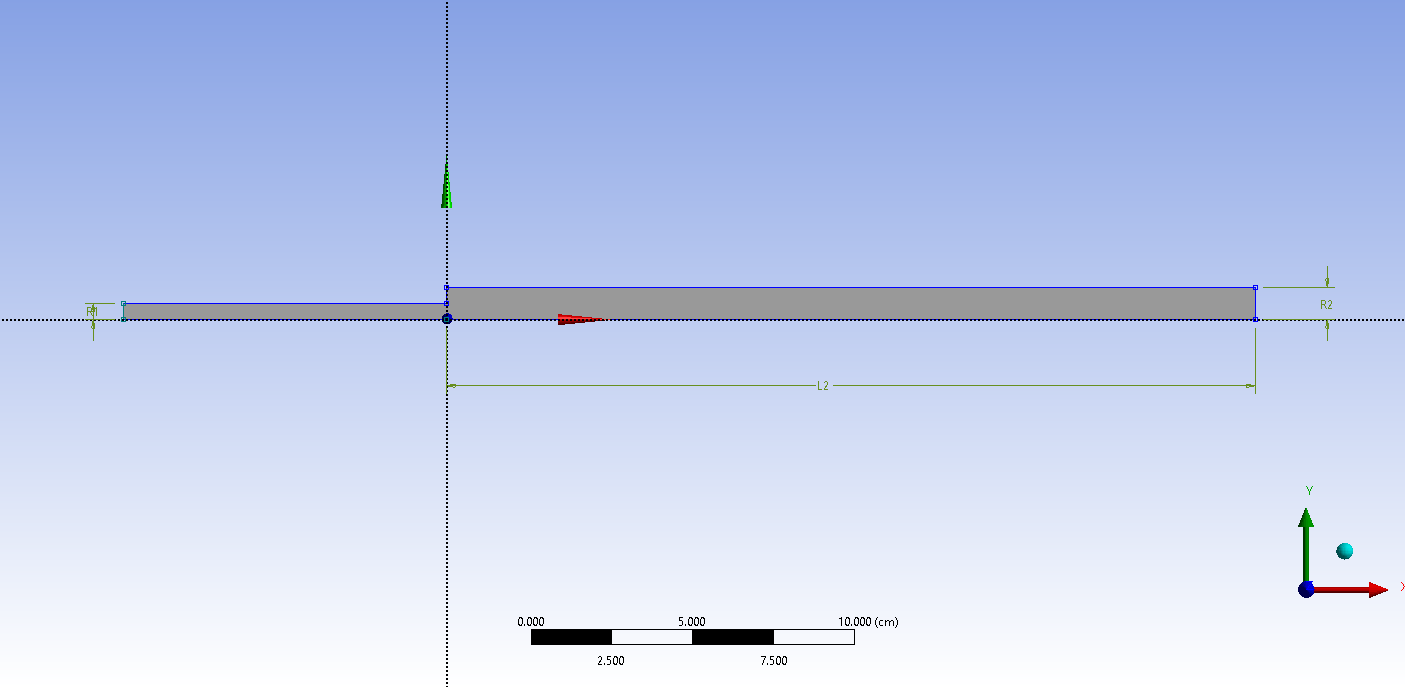
\includegraphics[width=14cm]{images/task1/sketch.png}
    \caption{Sketch of the geometry}
    \label{fig:sketch}
\end{figure}

%%%%%%%%%%% Conditions and Material Properties %%%%%%%%%%%%%%%%%%
\subsubsection{Conditions and Material Properties}
During the meshing part which will be further discussed on the following sections, named selections 
have been created and to be later used during the setup of the simulation.
CFD simulations are performed to see the behavior and change in properties of this given fluid of which its physical properties are taken to be density, $\rho = 100 \frac{kg}{m^{3}}$ and dynamic viscosity $\mu = 0.01 \frac{kg}{ms}. $\\

\noindent For this task, different values like the inlet velocity, density, inlet diameter and viscosity are chosen carefully to keep the Reynolds number of the flow under 2300, which ensures a laminar flow. The inlet velocity is set to be 0.554 m/s. The Reynolds number for this setup is calculated as follows:
\begin{equation} \label{eq:reynolds}
     Re = \frac{\rho * V_1 * (2R_1)}{\mu} = 55.4
\end{equation}
\\

\noindent The axisymmetric condition is selected with the lowermost edge being the symmetry axis and the remaining edges excluding the inlet and outlet are selected to be walls. Meaning that boundary conditions can be seen from Figure \ref{fig:boundary} where red lines show the inlet, yellows the outlet, greens the walls and the blue representing the symmetry axis. \\


\begin{figure}[h]
    \centering
    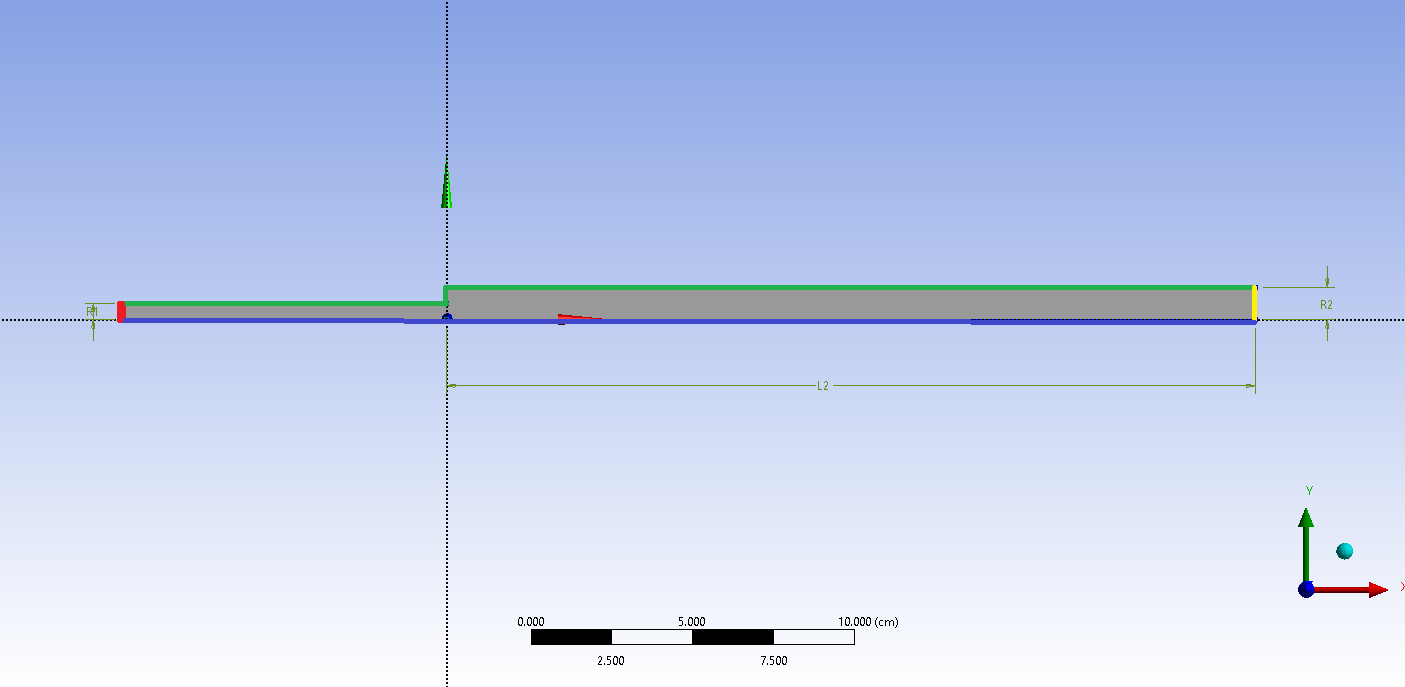
\includegraphics[width=15cm]{images/task1/sketch_paint.png}
    \caption{Boundary Conditions}
    \label{fig:boundary}
\end{figure}

\noindent When making the calculations, the laminar, axisymmetric flow parameters have been selected from the solver settings to represent the system properly and a Least Square based calculation is run.












%%%%%%%%%%%%%%%%%%%  %%%%%%%%%%%%%%%%%%%%



\end{task1}

\subsection{Task 2: Turbulent Flow Inside An Expanding Pipe}
\label{sec:task2}

This section revolves around the properties and analysis of a turbulent flow a fluid through an expansion. The same geometry and boundary conditions are used as the section before. However, some of the material properties and initial conditions have been changed to increase the Reynolds number to $10^5$ which results in a turbulent flow.\\

\noindent To accommodate this change, the viscosity of the fluid, $\mu$, has been decreased to $0.001 Pa.s$ while the density, $\rho$ has been increased to $10^3$ $kg/m^{3}$. Also, the inlet velocity has been upped from 0.554 to 10 $m/s$. Plugging these values into equation \ref{eq:reynolds}, we calculate the Re to be $10^5$. \\


\noindent In this analysis, two different simulations will be done using two different turbulence models below:
\begin{itemize}
    \item The $k - \epsilon$ model with standard model constants
    \item The $k - \omega$ model with standard model constants
\end{itemize}

\subsubsection{$k - \epsilon$ vs $k - \omega$ model}

While we are using two different turbulence models in our simulations, it is better to state their mechanisms from a higher level and compare their advantages over each other.\\

\noindent The $k-\epsilon$ model is one of the most popular methods to model turbulence. This model uses 2 transport equations to calculate K, the turbulent kinetic energy, and $\epsilon$, the turbulence dissipation rate. This relates to the kinetic energy transformed to heat caused by viscosity. Once these values are known, $\mu_t$, the turbulent viscosity is calculated and plugged in to the Navier-Stokes equations.\\

\noindent However, this model has its own disadvantages, especially near the system boundaries. This model needed damping functions near the boundaries which could get inaccurate easily. Also, it is not feasible in supersonic speeds, making it unpractical for areas like turbomachinery and aerodynamics. \\

\noindent To fill this gap, $k-\omega$ model is used. Unlike the former, this method uses $\omega$, which is the specific turbulence dissipation rate. Since this method does not utilize damping functions, it does not inherit the inaccuracies of them in the vicinity of system boundaries. This makes it a better model for near wall areas.

\subsection{Task 3: Pressure Loss Before and After the Expansion}
\label{sec:task3intro}

In this part, the pressure loss after sudden and gradual expansions will be examined for our geometry. 
While doing so, different expansion ratios will be considered and simulated. In these calculations, equations, materials and tables from Frank M. White's fluid mechanics textbook \cite{white_chul_2016} will be used frequently.\\


\noindent The minor loss measured by the head loss is defined \cite{white_chul_2016} as:

\begin{equation}
    h_m = \frac{\Delta p}{\rho g}
    \label{eq:hm}
\end{equation}

\noindent where $\rho$ is the density of the fluid, $g$ is the gravitational acceleration and $\Delta p$ is $p_1 - p_2$ with those being the pressure values before and after the expansion of the pipe. Also to be used in our calculations, minor head loss coefficient is calculated as follows:

\begin{equation}
    K = \frac{h_m}{V^2 / (2g)}
    \label{eq:headlosscoeff}
\end{equation}

\noindent where K is the average velocity inside the pipe, that is, the velocity we have defined when creating the inlet boundary conditions and initial conditions. \\

\noindent For the sudden expansion case where the expanding walls are perpendicular to the centerline of the pipe, 3 simulations are done for different expansion ratios, that is, the ratio of smaller pipes radius and that of the bigger pipe's. The ratios which will be examined are as follows:

\begin{itemize}
    \item 0.2
    \item 0.4
    \item 0.6
\end{itemize}

\noindent In addition to this, instead of a sudden expansion a gradual expansion with expansion ratio of 0.4 and a expansion degree (the angle between the centerline of the pipe and the expansion walls) of $2\theta = 20^{\circ}$.


\begin{figure}[H]
  \centering
  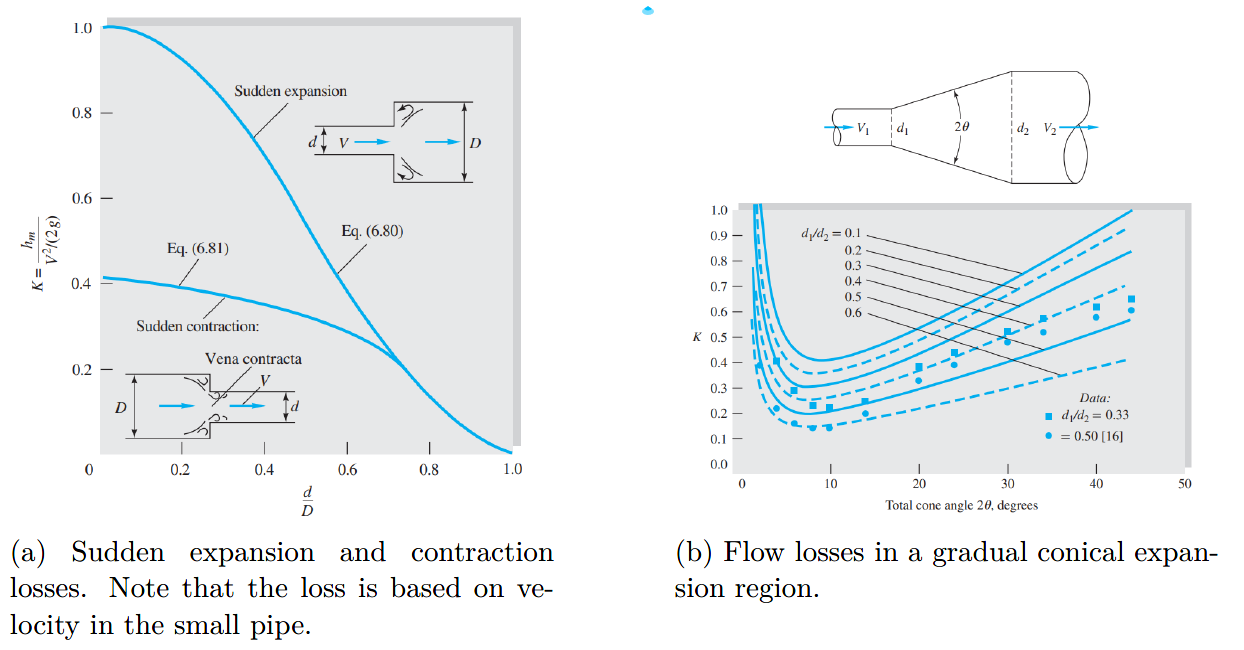
\includegraphics[width=.9\linewidth]{images/task3/expansion_figures.png}
  \caption{Expansion Plots \cite{white_chul_2016}}
  \label{fig:exp_plots}
\end{figure}


\noindent To validate and compare our results, plots that models these parameters from White's book \cite{white_chul_2016} will be used. Those plots can be seen from Figure \ref{fig:exp_plots}.




%%%%%%%%%%%%%%%%%%%% Results and Discussion %%%%%%%%%%%%%%%%%%%%%
\section{Results and Discussion}

\subsection{Task 1}
%%%%%%%%%%%%%%%%%% Grid Convergence %%%%%%%%%%%%%%%%%%%%
\subsubsection{Grid Convergence}
\noindent The geometry is modeled as an axisymmetric slice of the circular pipe using the Design Modeler tool of ANSYS Workbench. The same geometry is meshed into elements of different sizes to check whether the grid convergence is achieved or not. The element sizes tried to check convergence are as follows:

\begin{itemize}
    \item $10^{-2}$ meters
    \item $10^{-3} $ meters
    \item $5* 10^{-4}$  meters
\end{itemize}

\begin{figure}[h]
    \centering
    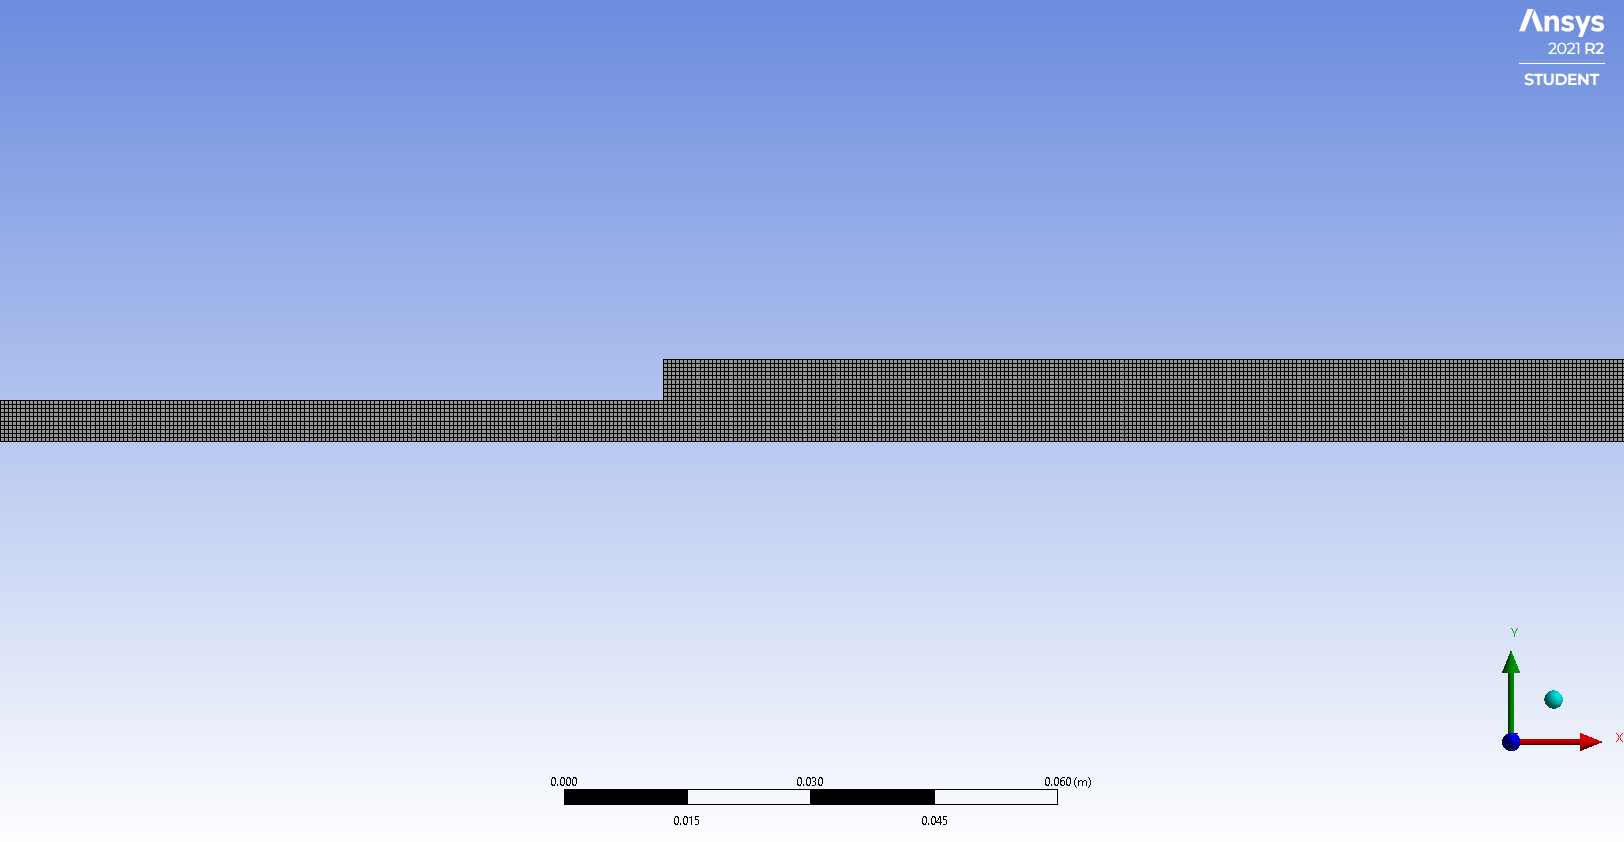
\includegraphics[width=16cm]{images/task1/5e04mesh.png}
    \caption{Mesh of the geometry with $5*10^{-4}$ meters as element size}
    \label{fig:mesh_fig}
\end{figure}


\noindent It was determined that after $5*10^{-4}$ meters of size, the results have been converged. For this condition, node and element numbers can be seen from Table \ref{table:mesh_info}, the mesh consisted of 12721 nodes and 12000 elements. While Figure \ref{fig:mesh_fig} shows the mesh from a broader perspective, Figure \ref{fig:closer_look} shows a zoomed view of the mesh created. Also, the student version of ANSYS struggled highly with smaller mesh sizes anyways.

\begin{table}[h]
\caption{Relevant Information On the Mesh}

\centering
\begin{tabular}{l|c}
\hline
\hline
Parameter          & Value                      \\ \hline
Element Size       & $5*10^{-4}m$ \\
Number of elements & 12000                      \\
Number of nodes    & 12721   

\end{tabular}

\label{table:mesh_info}
\end{table}


\begin{figure}[h]
    \centering{
    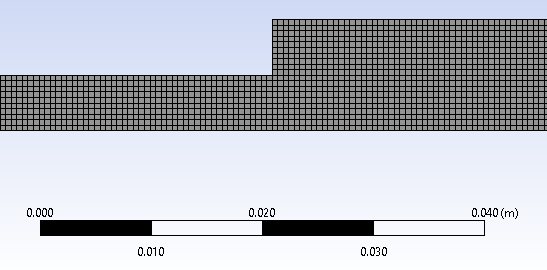
\includegraphics[width = 11cm]{images/task1/closer_look.png}
    \caption{A closer view of the mesh.}
    \label{fig:closer_look}}
\end{figure}


\noindent In order to conclude that the results have been converged, velocity profiles of the fluid at different cross-sections have been compared until little to no improvement on the results have been observed on results. As can be seen from Figure \ref{fig:convergence}, the results are almost the same between the element sizes of a and b. This relation is also closely observed on the velocity profiles from selected cross sections of the pipe.\\

\begin{figure}[H]

    \centering{
    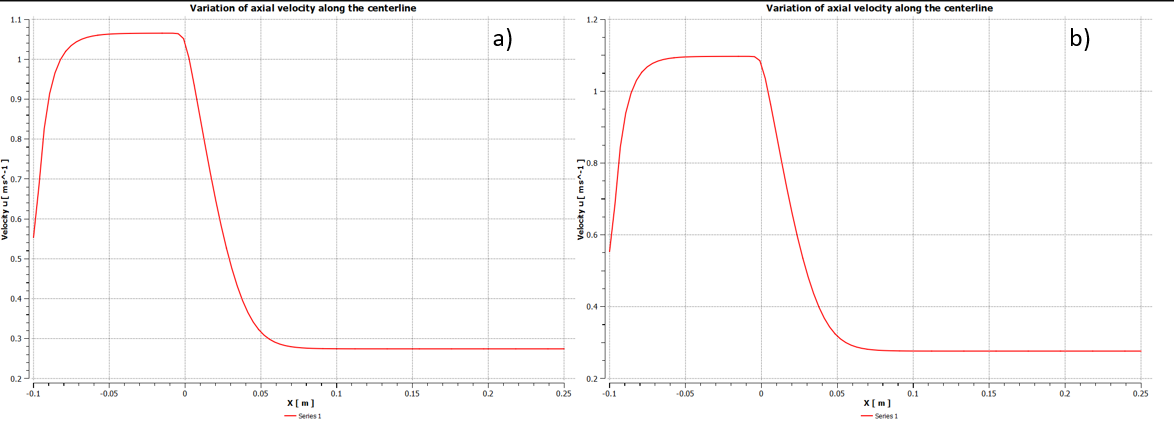
\includegraphics[width=16cm]{images/task1/convergence.png}
    \caption{Axial velocities along the centerline: a) Element size $10^{-3}$meters, b) Element size $5*10^{-4}$ meters.}
    \label{fig:convergence}}
\end{figure}

\noindent Figure \ref{fig:convergence2} shows the similarity between two different mesh sizes that have been tried and checked for grid convergence. The velocity profiles are taken from x=1cm for both cases. While Figure-\ref{fig:convergence2}.a is smoother, the results are almost exactly the same for both cases.

\begin{figure}[H]
    \centering{
    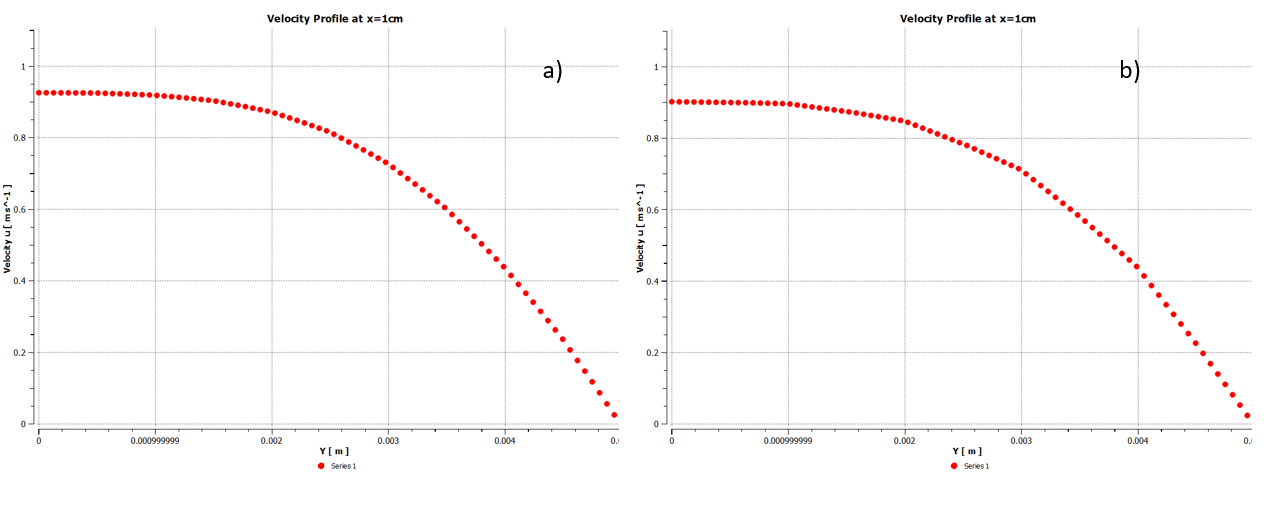
\includegraphics[width=14cm]{images/task1/convergence2.png}
    \caption{Comparison of the velocity profiles of element sizes at x=1cm shown on Figure \ref{fig:convergence}.}
    \label{fig:convergence2}}
\end{figure}


\noindent As requested from the project prompts, those 3 different mesh sizes are further compared by
plotting the axial velocity profiles at the axial locations of x = 0.5 cm, 1 cm,
1.5 cm, 2 cm, and 3 cm. Those plots can be seen from Figure \ref{fig:axials}. When compared, of course due to the difference in number of elements, finer mesh produces a smoother curve as expected since it contains more data points. However, the values kept at the same point are the same and the values are not changing with decreasing element size or increasing node count.


\begin{figure}[H]
    \centering
    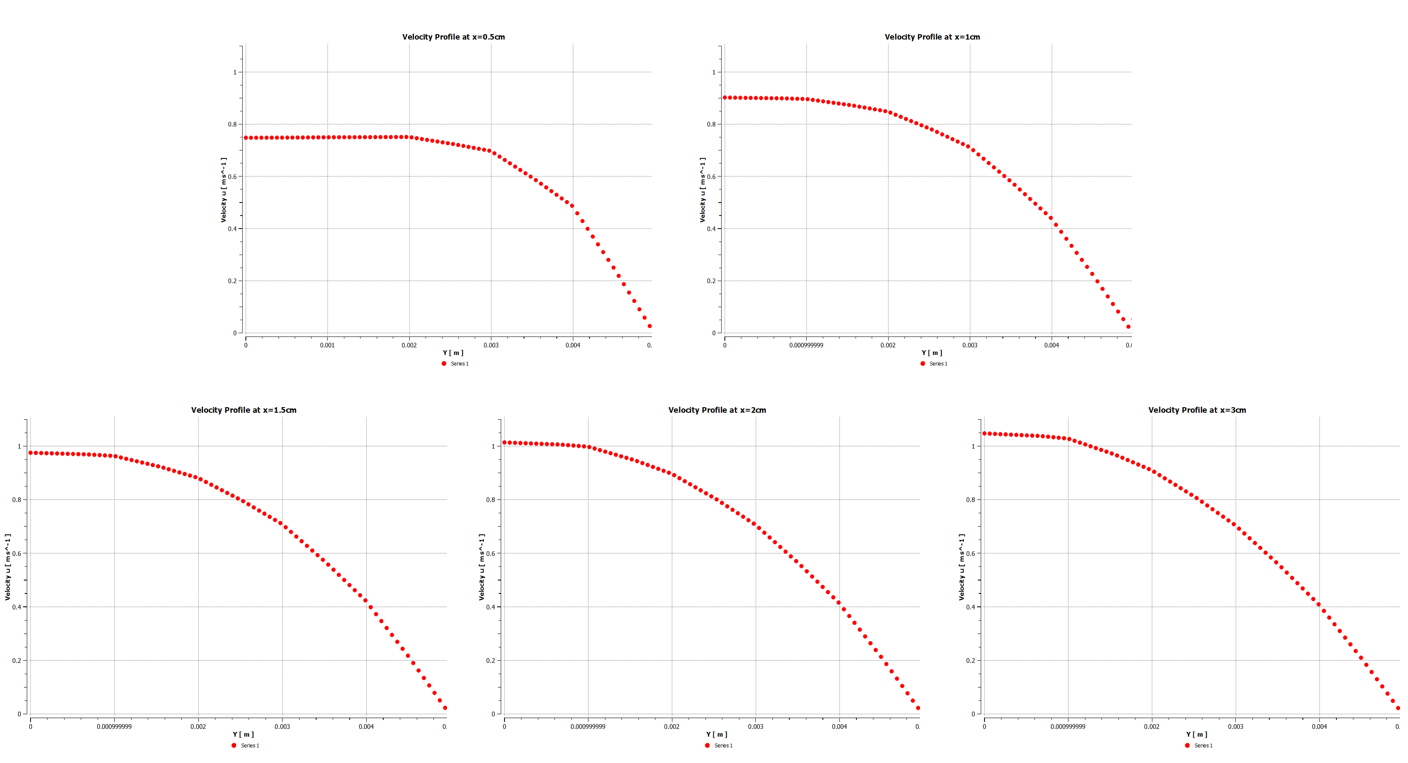
\includegraphics[width=15cm]{images/task1/e_03_total.png}
    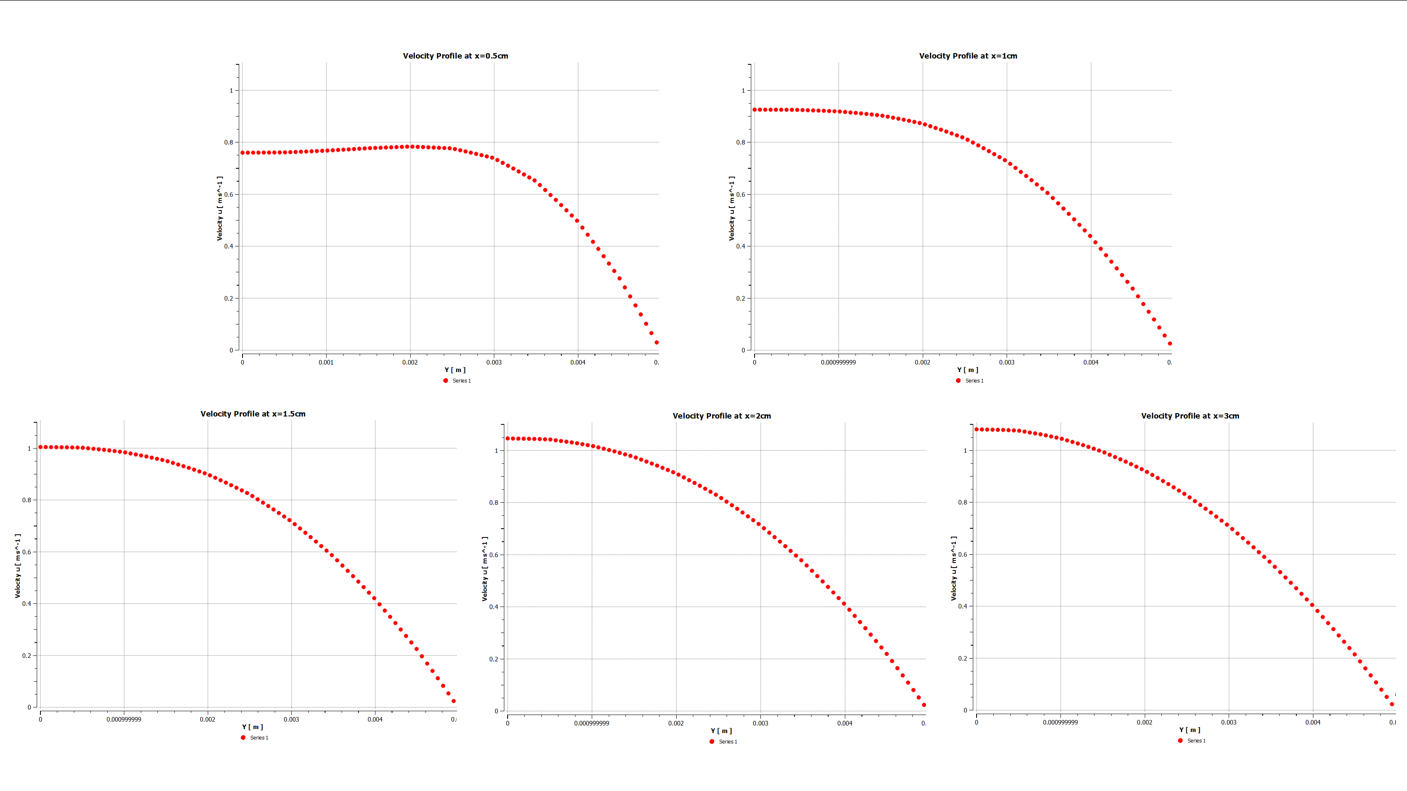
\includegraphics[width=15cm]{images/task1/5e_04_total.png}
    \caption{Velocity Profiles at x = 0.5, 1, 1.5, 2 and 3cm for element sizes $10^{-3}$m (above 5), and $5*10^{-4}$m (lower 5).}
    \label{fig:axials}
\end{figure}



%%%%%%%%%%%%%%% Residuals and Calculations %%%%%%%%%%%%
\subsubsection{Residuals and Calculations}
Once the calculation is run, we must be sure that a steady state condition is achieved. The reason for this check is due to nature of our solver and numerical methods used. Our solver stops the calculations on one of these two conditions:

\begin{itemize}
    \item Residual error in each step have dropped under a set threshold determined by the user and the solution is converged.
    \item Maximum number of steps have achieved.
\end{itemize}

\noindent A plot of the residuals have been drawn and can be seen on Figure \ref{fig:residuals}. As can be seen, 
all of the tracked values have gone under $10^{-6}$ which is low enough to state that a steady state has been achieved at the step.

\begin{figure}[H]
    \centering
    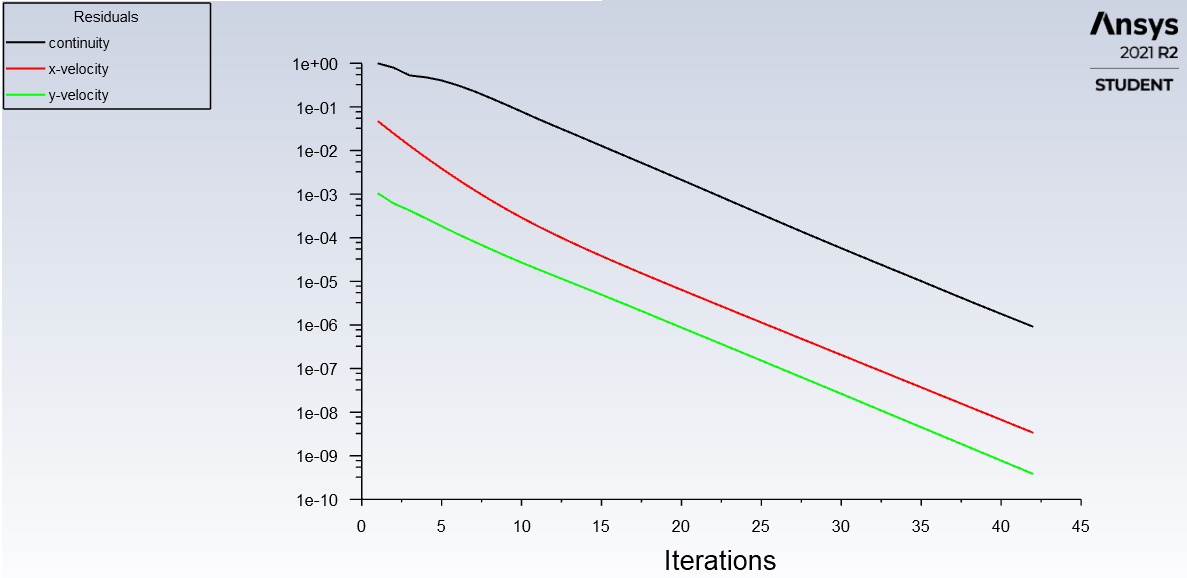
\includegraphics[width=15cm]{images/task1/residuals.png}
    \caption{Plot of the Residuals for Task 1}
    \label{fig:residuals}
\end{figure}
\\
\\
\noindent Velocity profiles at several cross sections along the centerline can be seen on Figure \ref{fig:velprof3}. This plot can be validated by using the \textbf{Poiseuille-Hagen} solution by using the formula given below. 

\begin{equation}
    u = 2V_{avg} * (1- \frac{r^{2}}{R^{2}})
    \label{eq:hagen}
\end{equation}
\\
\\
\noindent Where $V_{avg}$ is the average velocity of the fluid inside the pipe, $R$ is the radius of the pipe 
and the $r$ is the radial distance of the point from the centerline.

\begin{figure}[H]
    \centering
    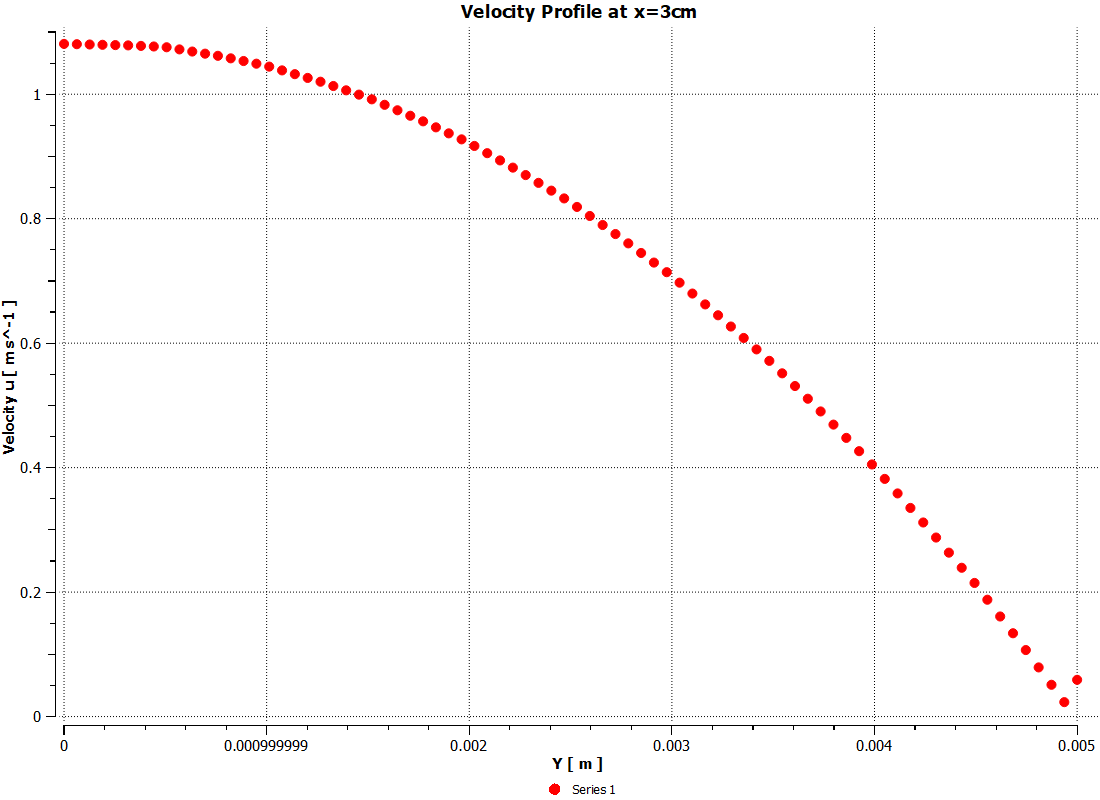
\includegraphics[width=14cm]{images/task1/vel_prof_3.png}
    \caption{Velocity Profile at x=3cm}
    \label{fig:velprof3}
\end{figure}

\noindent While not perfect, it can be clearly said that our simulation solution agrees with the given theoretical equations used to model these flows. When we plug in the values to equation \ref{eq:hagen}, we obtain the following solution:

\[ 2*0.554m/s * \Big(1 - \frac{0}{0.1^{2}m^{2}}\Big) = 1.108 m/s \] 

\noindent when evaluated at the centerline. This value is \textbf{within $1\%$} of the value we obtained from the simulation. A similar picture is seen when looked at the axial velocity profiles along the centerline of the pipe. A plot can be seen from Figure \ref{fig:axial}, the values are again in agreement with the theoretical values and become closer as the boundary layer is formed throughout the length of the pipe. 

\begin{figure}[H]
    \centering
    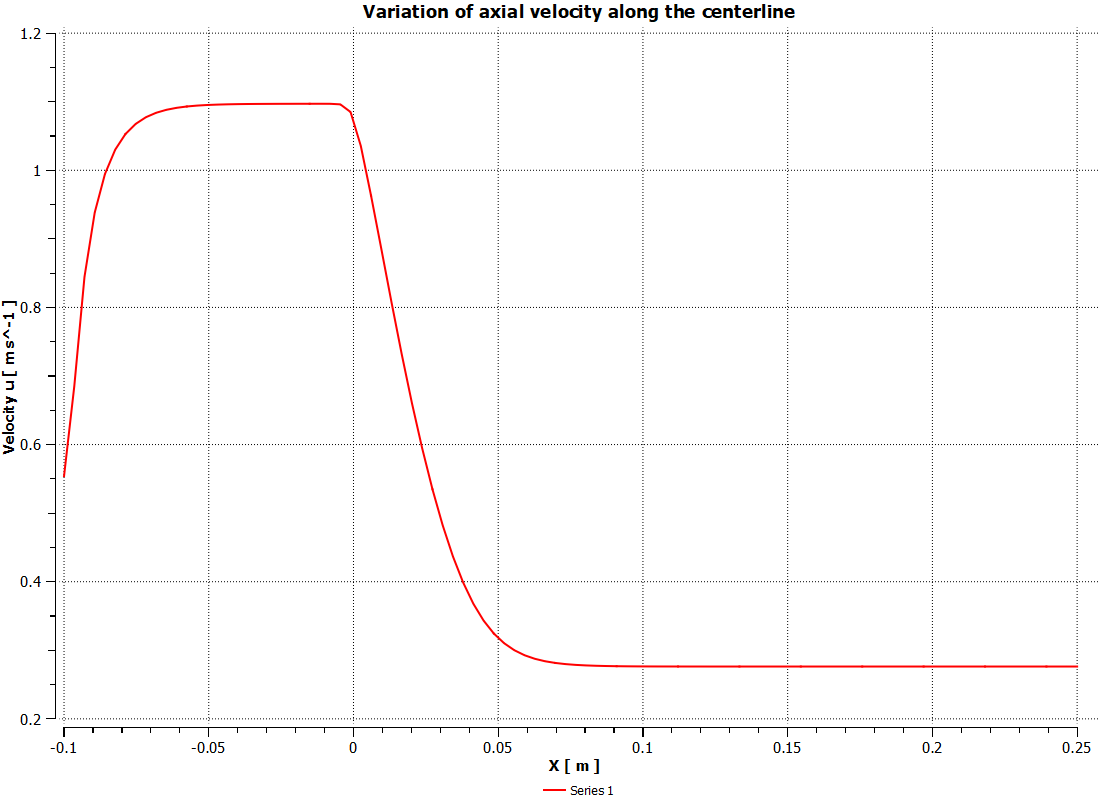
\includegraphics[width=15cm]{images/task1/axial.png}
    \caption{Axial velocities along the centerline}
    \label{fig:axial}
\end{figure}

\noindent To further show the validation of the results, velocity profiles at $x=5$ and $x=7.5$cm have been plotted which can be seen from Figure \ref{fig:vel_profiles_hagen}. Also, using MATLAB, velocity profile at x=5cm have been plotted with the Hagen equation on the same plot to show how close the data are to each other on Figure \ref{fig:matlab_hagen}.




\begin{figure}[H]
 \centering
\begin{subfigure}{.5\textwidth}
  \centering
  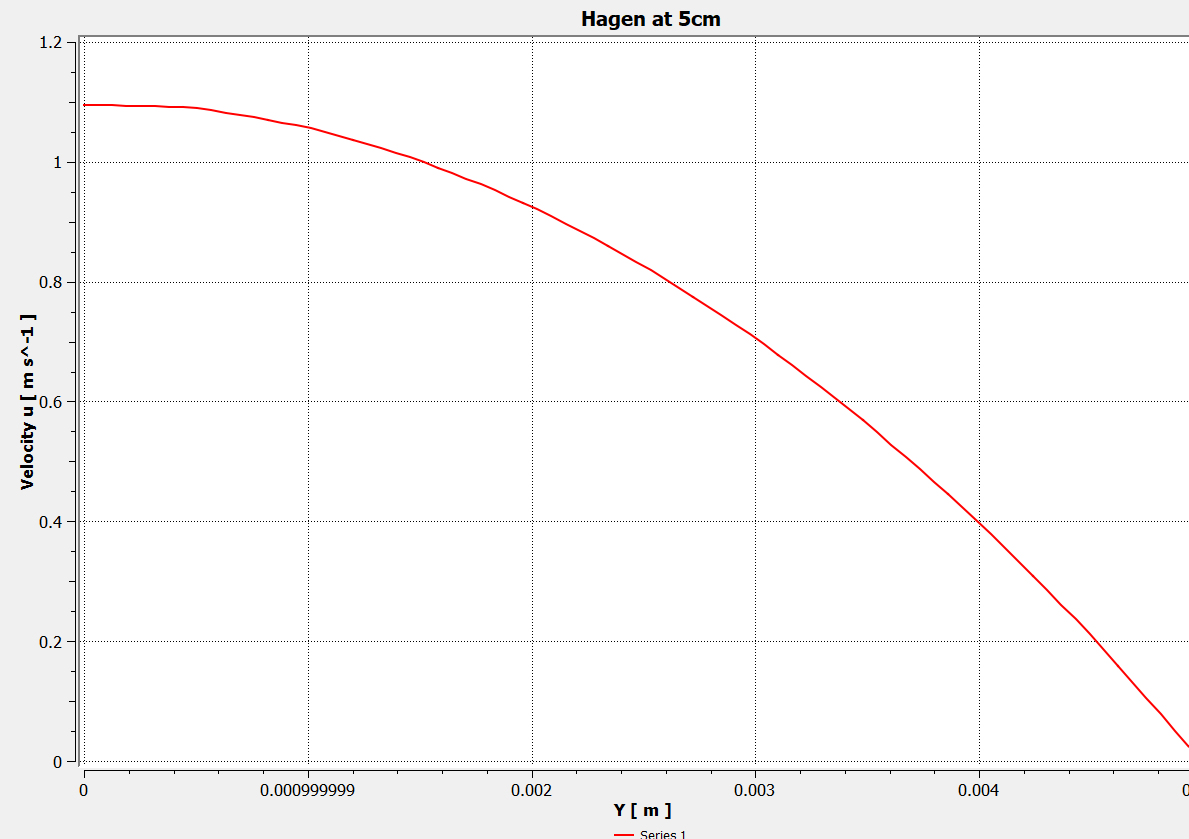
\includegraphics[width=.9\linewidth]{images/task1/hagen5.png}
  \caption{Velocity Profile at x=5cm}
  \label{fig:velprof5cm}
\end{subfigure}%
~
\begin{subfigure}{.5\textwidth}
  \centering
  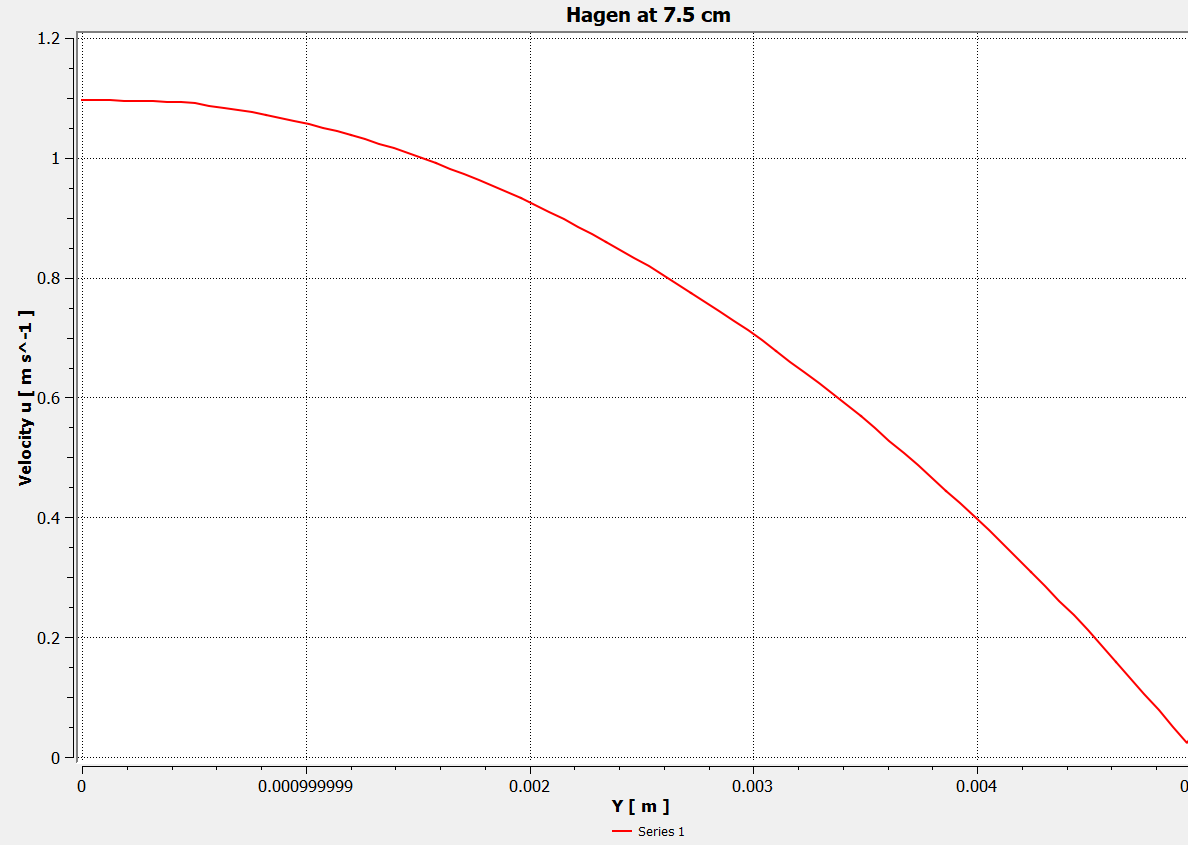
\includegraphics[width=.9\linewidth]{images/task1/hagen75.png}
  \caption{Velocity Profile at x=7.5cm}
  \label{fig:velprof75cm}
\end{subfigure}
~
\begin{subfigure}{.45\textwidth}
  \centering
  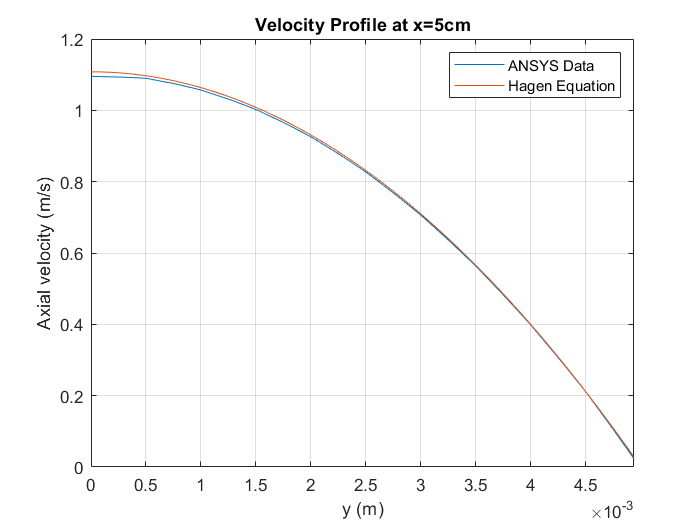
\includegraphics[width=.9\linewidth]{images/task1/hagen_ansys.png}
  \caption{My velocity profile vs the Poiseuille-Hagen equation at x=5cm}
  \label{fig:matlab_hagen}
\end{subfigure}
~
\begin{subfigure}{.45\textwidth}
  \centering
  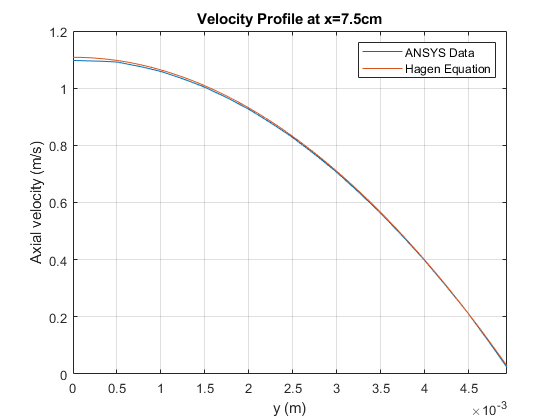
\includegraphics[width=.9\linewidth]{images/task1/hagen75_1.png}
  \caption{My velocity profile vs the Poiseuille-Hagen equation at x=7.5cm}
  \label{fig:matlab_hagen2}
\end{subfigure}
\caption{Velocity profiles and analytical comparisons}
\label{fig:vel_profiles_hagen}
\end{figure}

%%%%%%%%%%%%%%% Contours and Streamlines %%%%%%%%%%%%
\subsubsection{Contours and Streamlines}
Another useful way of interpreting the results is by visualising the obtained data into different kinds of contours and using streamlines that represent the flow inside the pipe. Using the post-processing tools of ANSYS, I have plotted the pressure contour and streamlines both separately and on top of each other. Which can be seen on Figures \ref{fig:stream} and \ref{fig:stream_w_pressure}.

\begin{figure}[H]
    \centering
    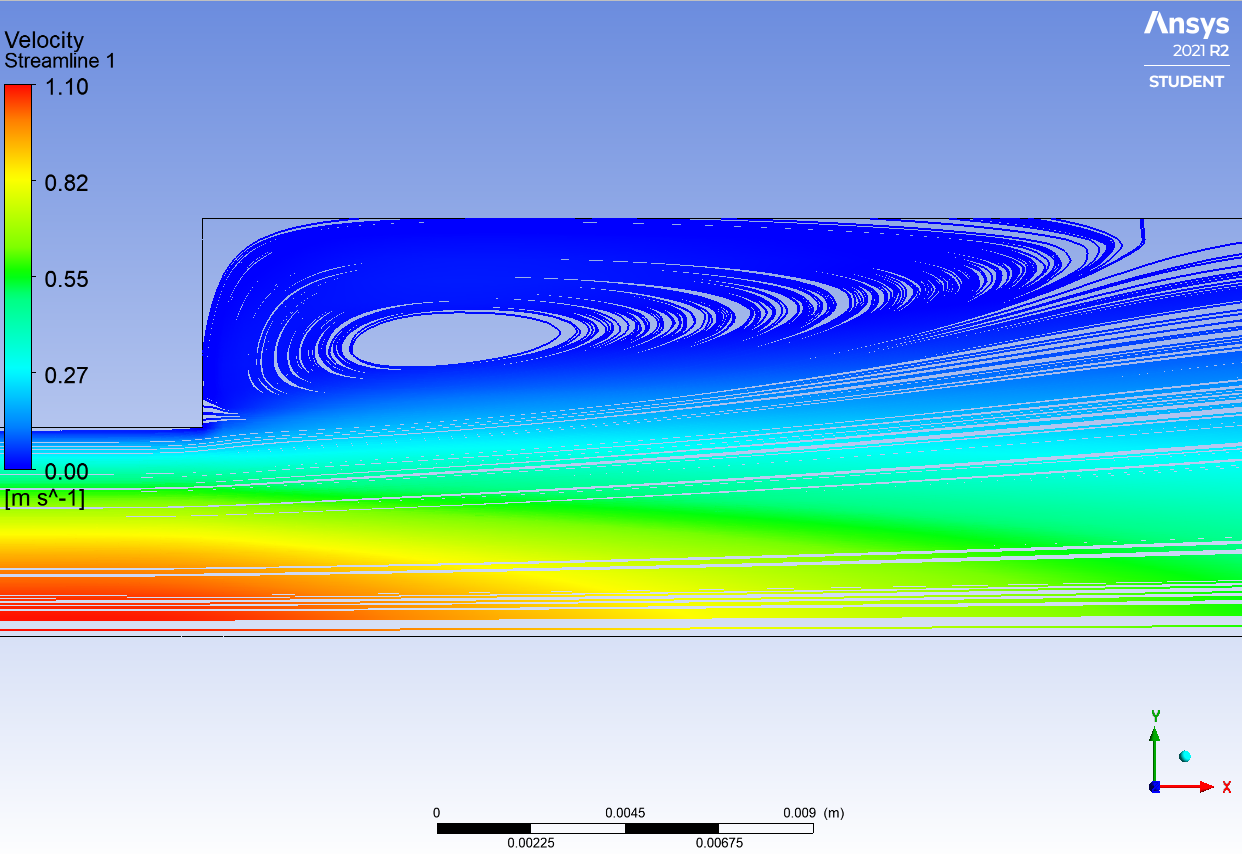
\includegraphics[width=0.9\textwidth]{images/task1/streamlines.png}
    \caption{Streamlines for the flow}
    \label{fig:stream}
\end{figure}

\begin{figure}[H]
    \centering
    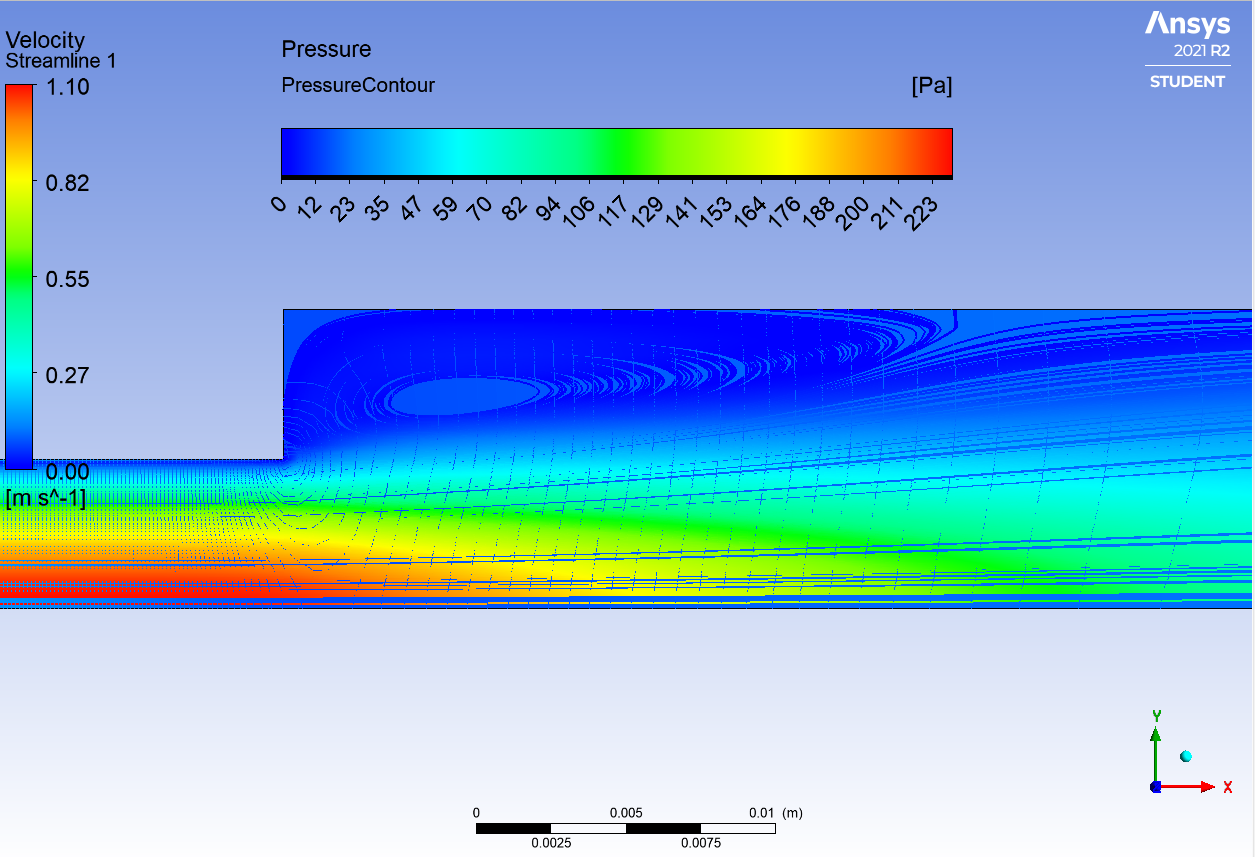
\includegraphics[width=0.9\textwidth]{images/task1/streamline_w_pressure.png}
    \caption{Streamlines for the flow plotted with pressure contours}
    \label{fig:stream_w_pressure}
\end{figure}

\noindent The streamlines for the recirculation zone can be clearly seen from the figures. This recirculation is induced by the expansion of the pipe. As the expansion causes a reduction on the pressure of the pressure at shown places, fluid particles at that point start to recirculate. \\

\noindent As expected, velocity is maximum in the centerline of the smaller pipe and pressure starts higher with the flow and dropping especially after the expansion. This drop in pressure is caused by the turbulent mixing of the flow where the pipe expands, which causes a decrease in mechanical energy.


%%%%%%%%%%%%%%% Experimental Comparison %%%%%%%%%%%%
\subsubsection{Experimental Comparison}
Now that we have made some comparisons of our results with theoretical models and equations. It is the next step to validate our results by comparing them with data obtained from previous experimental studies. To achieve this, we will be using an article published by Hammad et al.\cite{hammad_ötügen_arik_1999}. In their study, they also observed and analized the flow of a fluid through an expanding pipe.

\begin{figure}[H]
 \centering
\begin{subfigure}{.7\textwidth}
  \centering
  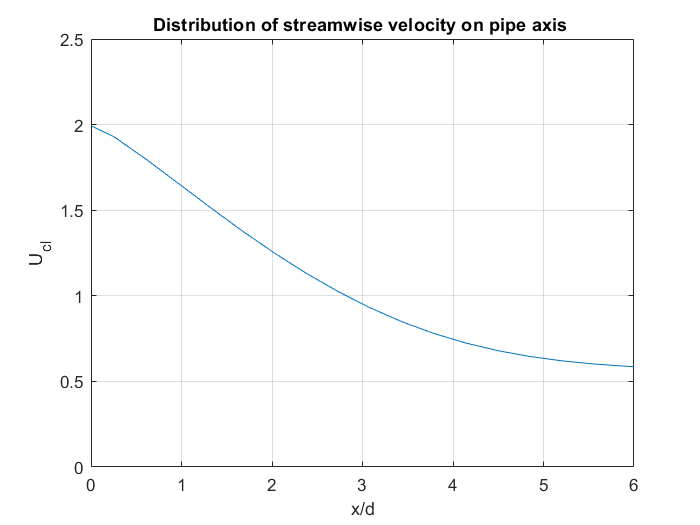
\includegraphics[width=.7\linewidth]{images/task1/x_d_norm.png}
  \caption{Distribution of streamwise velocity on pipe axis of ANSYS data.}
  \label{fig:x_d_norm}
\end{subfigure}%

\begin{subfigure}{.8\textwidth}
  \centering
  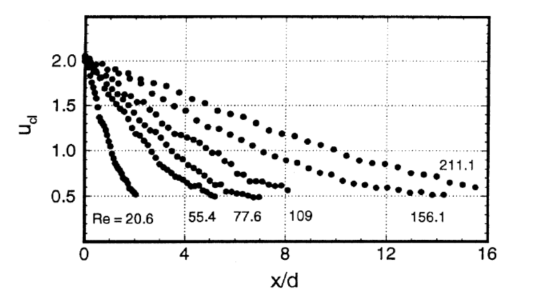
\includegraphics[width=.9\linewidth]{images/task1/x_d_norm_actual.png}
  \caption{Distribution of streamwise velocity on pipe axis from Hammad et al.\cite{hammad_ötügen_arik_1999}}
  \label{fig:x_d_norm_actual}
\end{subfigure}

\caption{Streamwise Velocity Comparison}
\label{fig:xd_norm}
\end{figure}

\noindent Figure \ref{fig:xd_norm} shows the similarities with data from our simulation and the data provided by \cite{hammad_ötügen_arik_1999}. While their chart contains data points from 6 different flows with different Reynolds numbers, the one which $Re = 55.4$ corresponds to our MATLAB plot that is shown above with very little error. This distribution makes sense since the fluid enters the second pipe with the highest velocity that is obtained from the equation \ref{eq:hagen} and that value corresponds to twice of the average velocity of the fluid. However, as the fluid moves deeper into the second pipe, the velocity at the centerline drops to around half of the average velocity.\\


\noindent Moreover, Hammad et al. provides velocity vectors for the case of $Re = 55.4$ throughout the length of the wider pipe. Once we obtain the velocity vector plots from ANSYS Fluent ourselves, a comparison can be made between our simulated data and their experimental data. 

\begin{figure}[H]
 \centering
\begin{subfigure}{.8\textwidth}
  \centering
  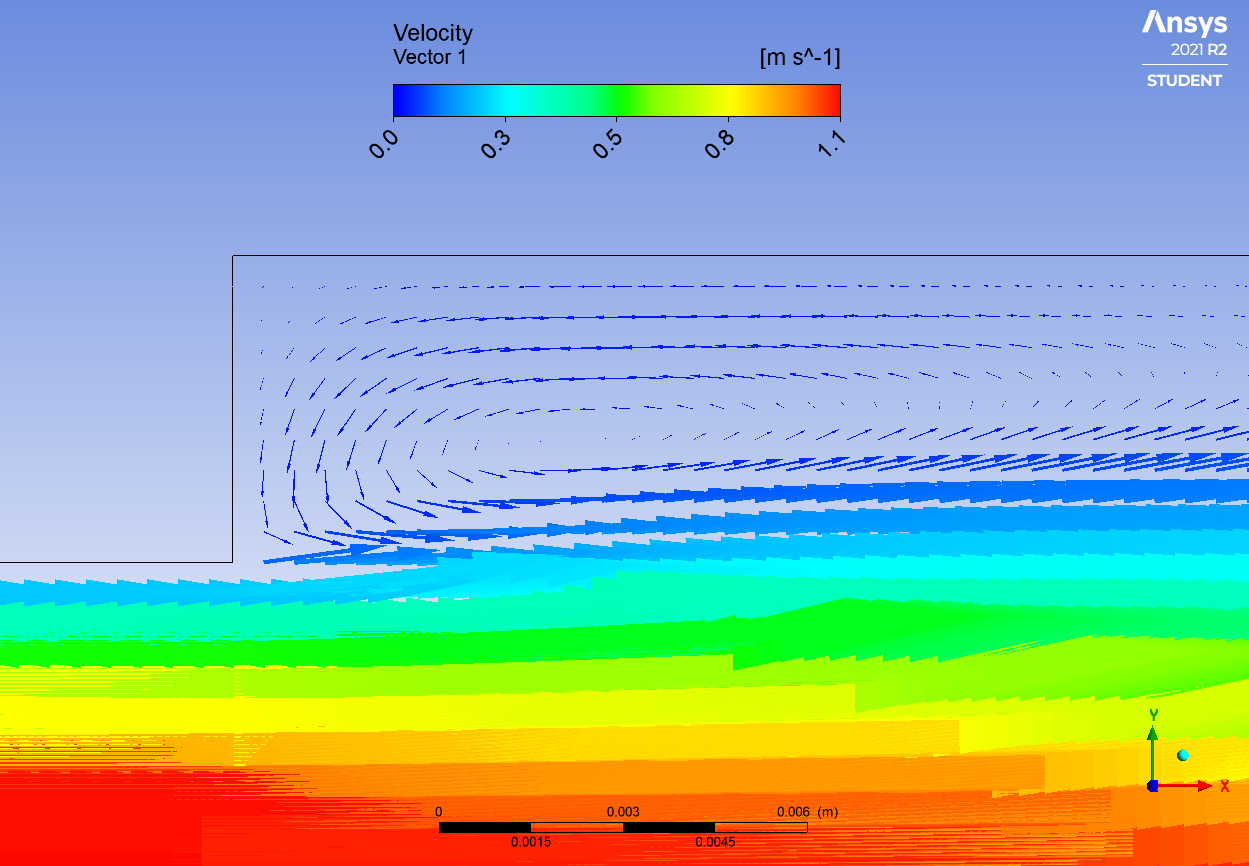
\includegraphics[width=.8\linewidth]{images/task1/vectors.png}
  \caption{Upscaled velocity vectors at the expansion.}
  \label{fig:vel_vel1}
\end{subfigure}%
\hfill
\begin{subfigure}{.8\textwidth}
  \centering
  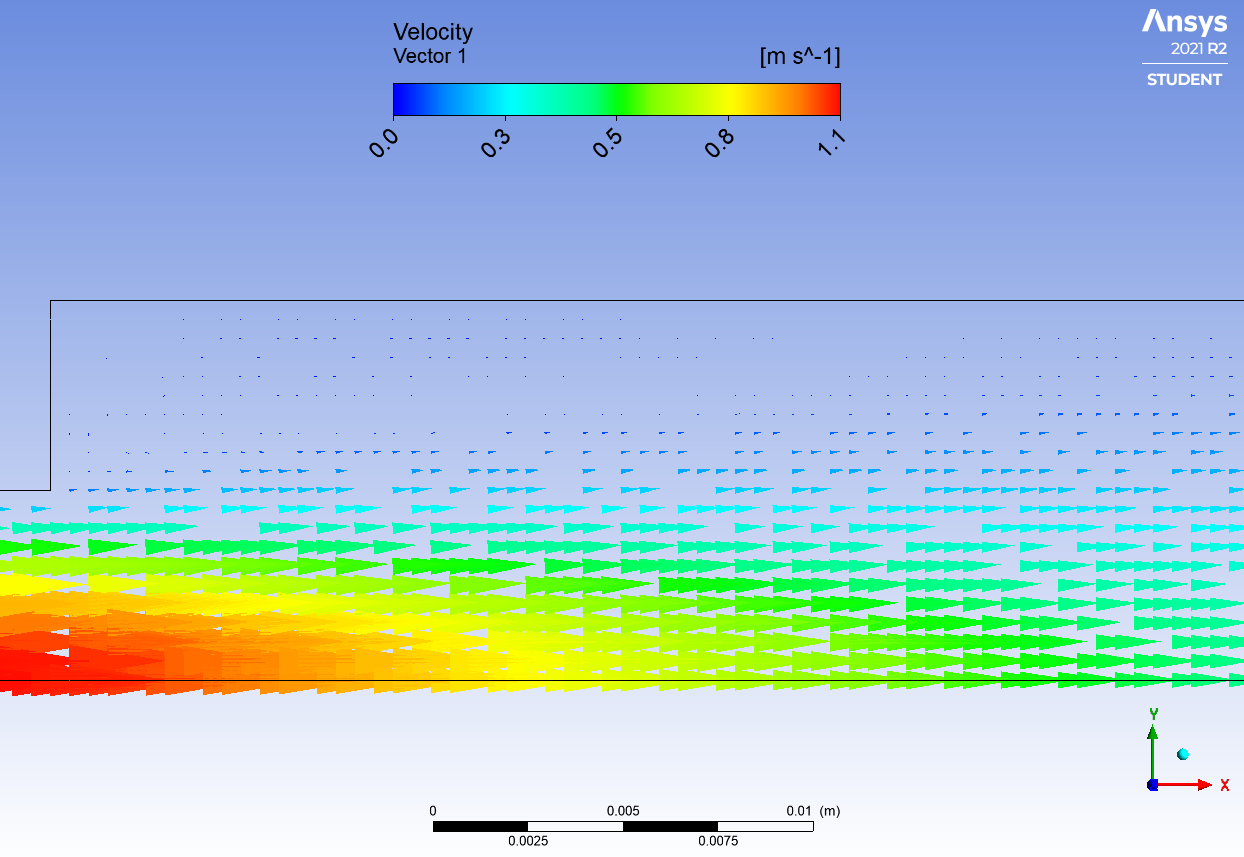
\includegraphics[width=.8\linewidth]{images/task1/vectorsplot.png}
  \caption{Velocity vectors at the expansion.}
  \label{fig:vel_vel2}
\end{subfigure}
\hfill
\begin{subfigure}{.8\textwidth}
  \centering
  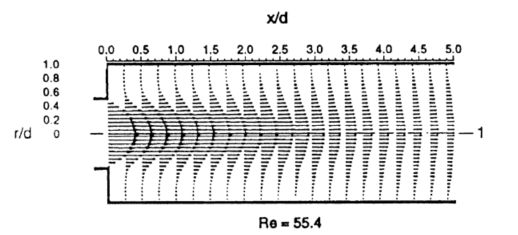
\includegraphics[width=.9\linewidth]{images/task1/vel_vectors.png}
  \caption{Measured velocity vectors from Hammad et al.\cite{hammad_ötügen_arik_1999}}
  \label{fig:vel_vel_measured}
\end{subfigure}

\caption{Streamwise Velocity Comparison}
\label{fig:vel_vec_comp}
\end{figure}

\vspace{0.5cm}
\noindent As can be seen from Figure \ref{fig:vel_vec_comp}, the measured values from the study and our Fluent simulation are in agreement. They both have maximum magnitude at the centerline and the magnitude gets smaller as the position of the vector gets farther away from the centerline. Also, as $x/d$ increases, magnitude of the vectors on the centerline decreases for both cases.
\\

\noindent Another aspect that was observed and modeled by Hammad et al. is the reattachment length of around the recirculation zone. In our case, the reattachment length is found looking at the streamlines and finding the point at which a streamline connects to the wall. The part before the reattachment point is called the recirculation zone. For this experiment, reattachment points have been found and plotted for 4 different $Re$ values. The change in the $Re$ values are made possible by changing the inlet velocities. Tested $Re$ values are 30, 55.4, 100 and 150.\\



\noindent The determination of the locations of the reattachment points is shown in Figure \ref{fig:reattach}. For all different cases, finding the reattachment point required tinkering with the number of streamlines to be drawn since in some cases. This was due to the fact that the location of the reattachment point was dependent on the concentration of the streamlines. The crosshairs and highlighted points on Figure \ref{fig:reattach}, depict the decided positions of reattachment points.


\begin{table}[H]
\caption{Reattachment lengths for Reynolds numbers}
\centering
\begin{tabular}{c|c}
\hline
Reynolds Number & Reattachment Length (m) \\ \hline
30              & 0.0141                  \\
55.4            & 0.0236                  \\
100             & 0.0430                  \\
150             & 0.0681                 
\end{tabular}
\end{table}

\noindent These numbers do follow the trendline that Hammad et al. has shown in their study and this can be shown by plotting our points over their chart, which can be seen from Figure \ref{fig:reattach_plot}. In this plot, our data points are shown with green circles. 

\begin{figure}[H]
    \centering
    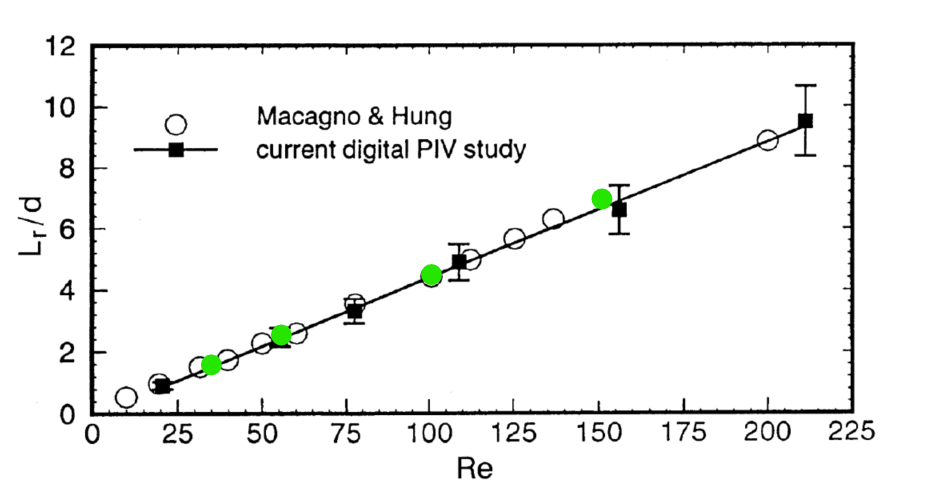
\includegraphics[width=14cm]{images/task1/reattach_plot.png}
    \caption{Plot of simulated reattachment lengths over the model of Hammad et al.}
    \label{fig:reattach_plot}
\end{figure}



\begin{figure}[H]
 \centering
\begin{subfigure}{.5\textwidth}
  \centering
  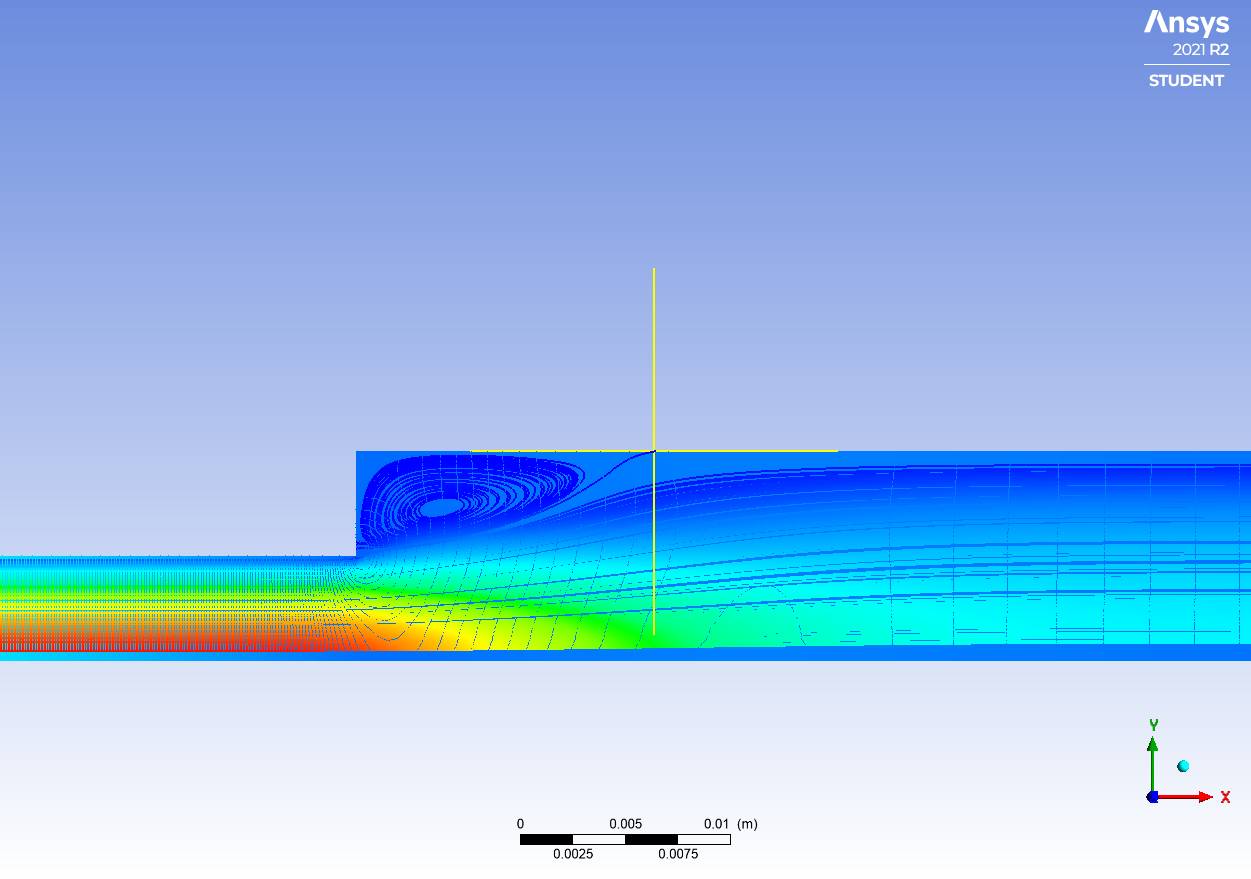
\includegraphics[width=.95\linewidth]{images/task1/030_attachement_0_0141.png}
  \subcaption{}
  \label{fig:reat_a}
\end{subfigure}%
\hfill
\begin{subfigure}{.5\textwidth}
  \centering
  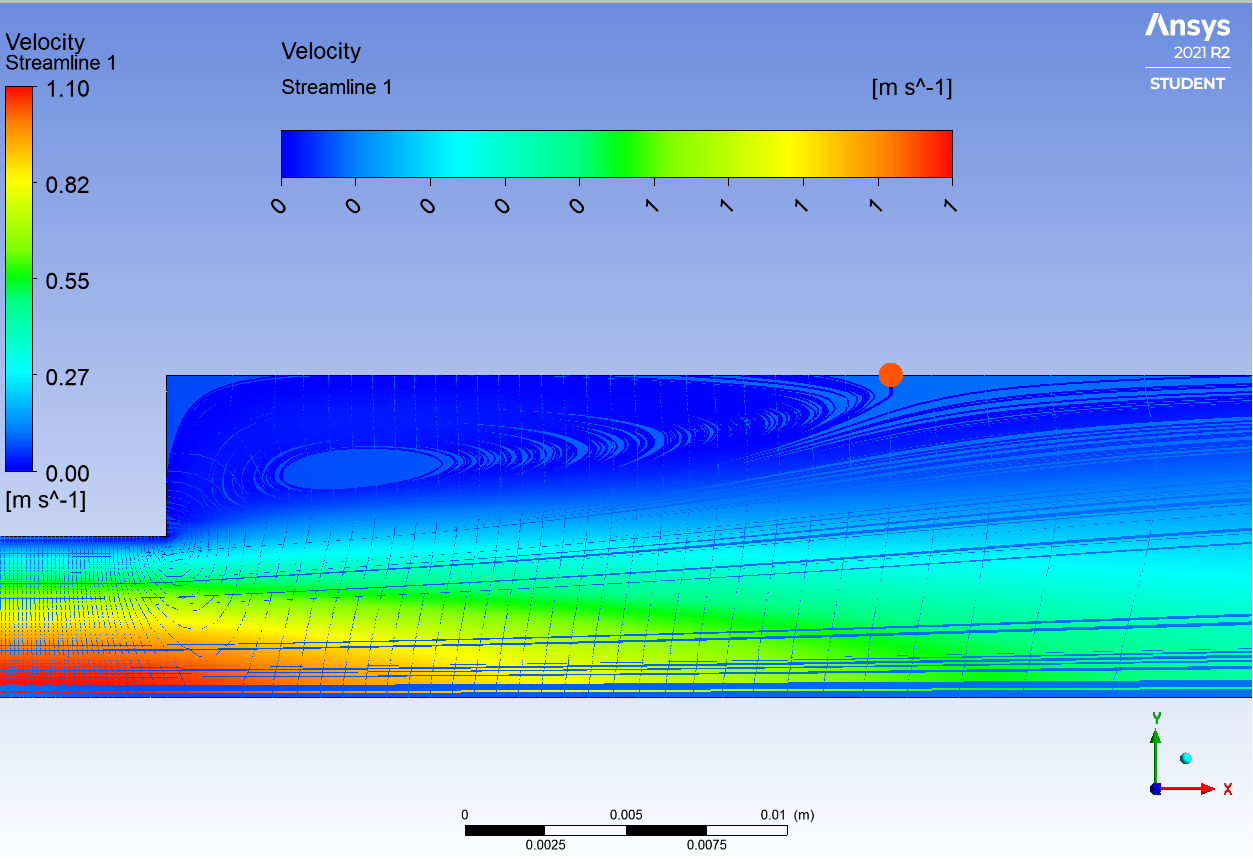
\includegraphics[width=.95\linewidth]{images/task1/0554_attachement_0_0236.png}
  \subcaption{}
  \label{fig:reat_b}
\end{subfigure}
\hfill
\begin{subfigure}{.75\textwidth}
  \centering
  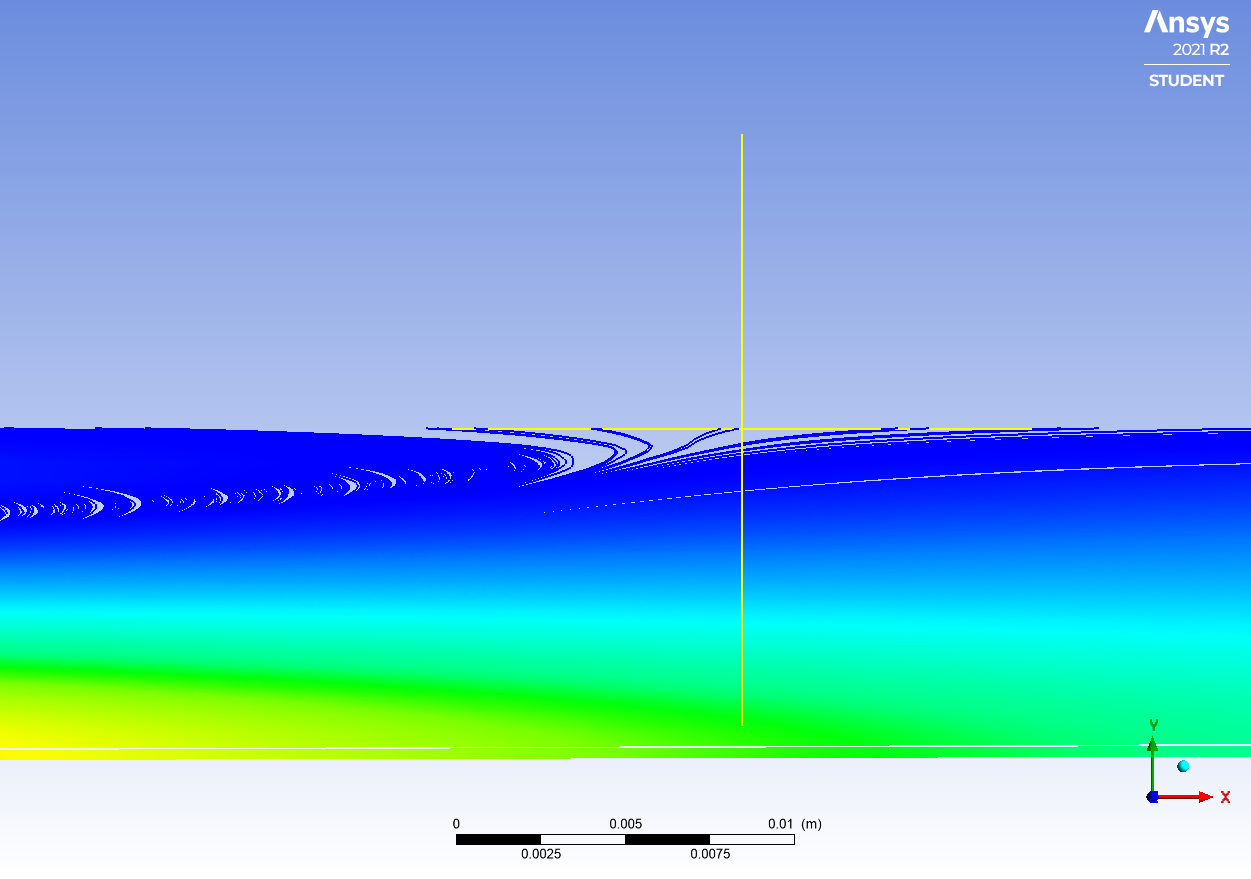
\includegraphics[width=.95\linewidth]{images/task1/100_attachement_0_430.png}
  \subcaption{}
  \label{fig:reat_c}
\end{subfigure}
\hfill
\begin{subfigure}{.75\textwidth}
  \centering
  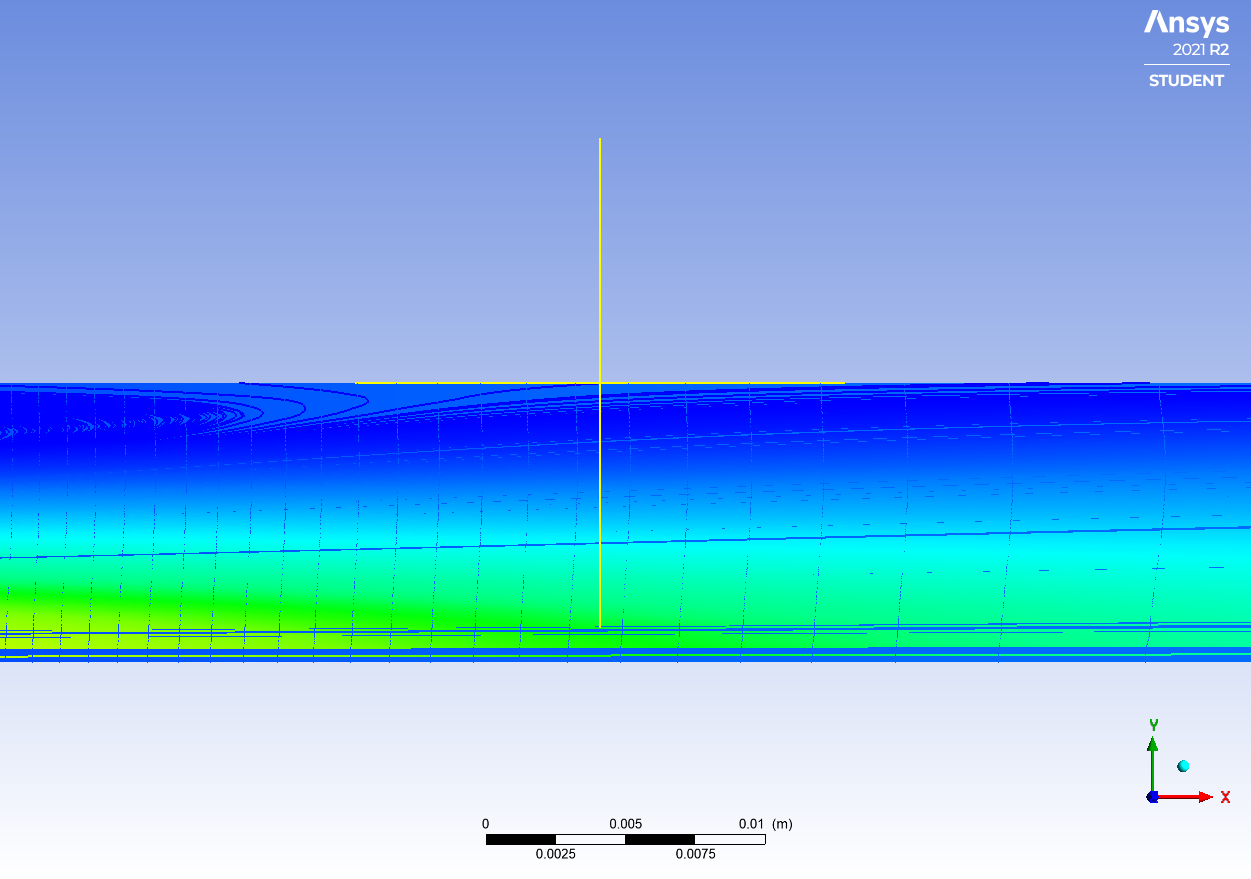
\includegraphics[width=.95\linewidth]{images/task1/150_attachement_0_0681.png}
  \subcaption{}
  \label{fig:reat_d}
\end{subfigure}
\caption{Reattachment Points for 4 different Reynolds numbers.}
\label{fig:reattach}
\end{figure}





\subsection{Task 2}
\label{sec:task2results}


The main differences between the $k-\epsilon$ and $k-\omega$ models have been discussed in section \ref{sec:task2}. In this section, their results for this specific case will be examined and compared. Especially, the recirculation zone and the vicinity of the expansion of the pipe will be studied.\\

\noindent While the same sketches and geometry is used from Task 1, also, grid convergence is achieved at the same mesh sizes as before. The mesh that was sufficiently fine was found when the element size was set to $5*10^{-4}$ meters. An image of this mesh can be seen from Figure \ref{fig:task2mesh}. Also, to confirm the achievement of steady state conditions, the residuals have been plotted an shown in Figure \ref{fig:task2_residuals}.

\begin{figure}[H]
    \centering
    \begin{subfigure}{.45\textwidth}
    \centering
    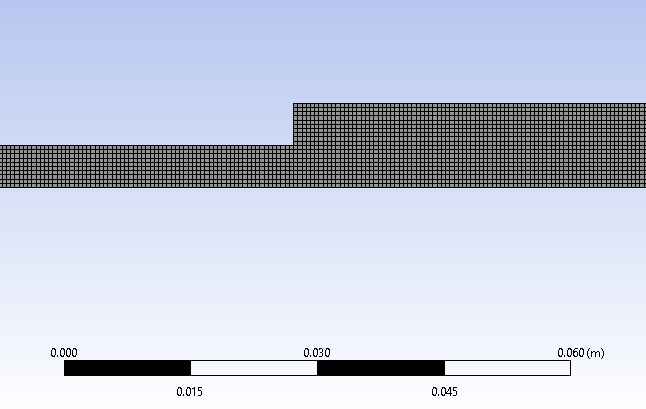
\includegraphics[width=.95\linewidth]{images/task2/task2-1/task2_mesh.png}
    \caption{Mesh for both models}
    \label{fig:task2mesh}
    \end{subfigure}
\hfill
\begin{subfigure}{.45\textwidth}
    \centering
    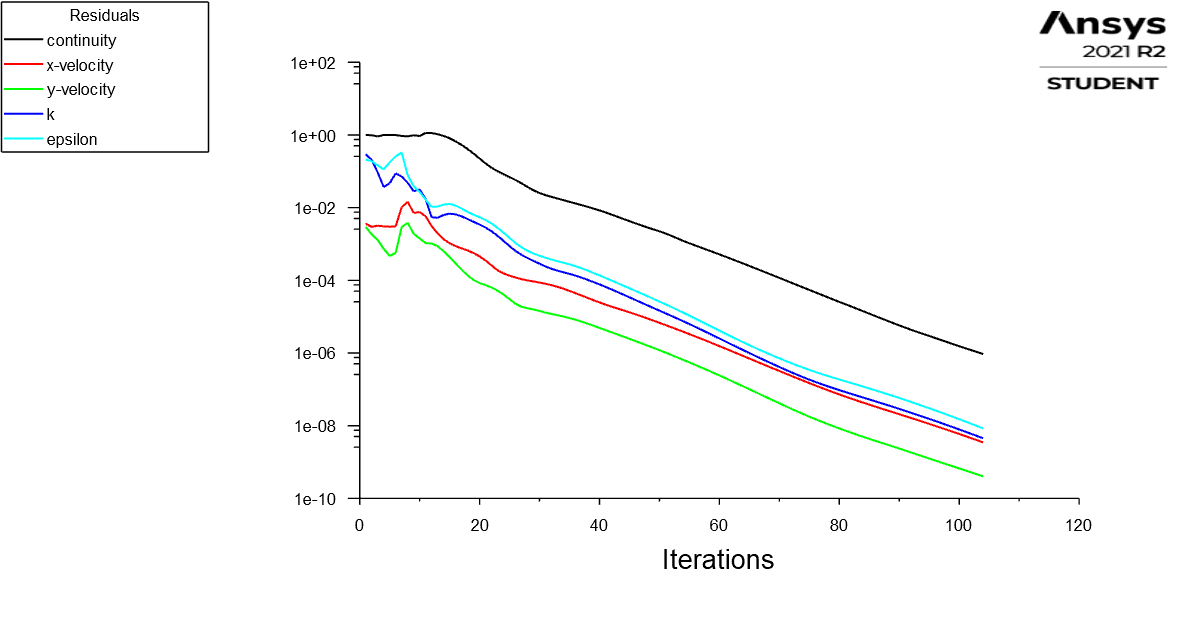
\includegraphics[width=.95\linewidth]{images/task2/task2-1/task2_1residuals.png}
    \caption{Residual plot for the models}
    \label{fig:task2_residuals}
\end{subfigure}
    
    \hfill
    \caption{Residuals and Mesh Sizes}
\end{figure}

\noindent Following this validation of the results. Also, the inlet and outlet fluxes have been compared and it was found that their difference was in the order of $10^{-9}$. Therefore, since we have shown that our simulation is seemingly meaningful, now I will be continuing with the comparisons of the models, starting with the velocity profiles.\\

\subsubsection{Comparison of the Velocity Profiles}

\noindent As can be seen from Figure \ref{fig:axial_task2}, while the main behavior is quite similar, there are deviations between the axial velocity profiles along the centerline. Specifically, there is a sudden and steep decrease in velocity after the expansion in both cases, however, this steep decrease is more delayed in the $k-\omega$. This feature clearly indicates a bigger recirculation zone and hints a longer reattachment length for the $k-\omega$ model. Besides this, the profiles are quite similar.\\


\noindent After this, velocity profiles from various cross sections have been gathered to be compared. The specific locations of those cross sections are shown with yellow lines in Figure \ref{fig:task2cross}. Particularly, these cross sections are taken from those that are inside or in the vicinity of the recirculation zone.\\

\begin{figure}[H]
    \centering
    \begin{subfigure}{.45\textwidth}
    \centering
    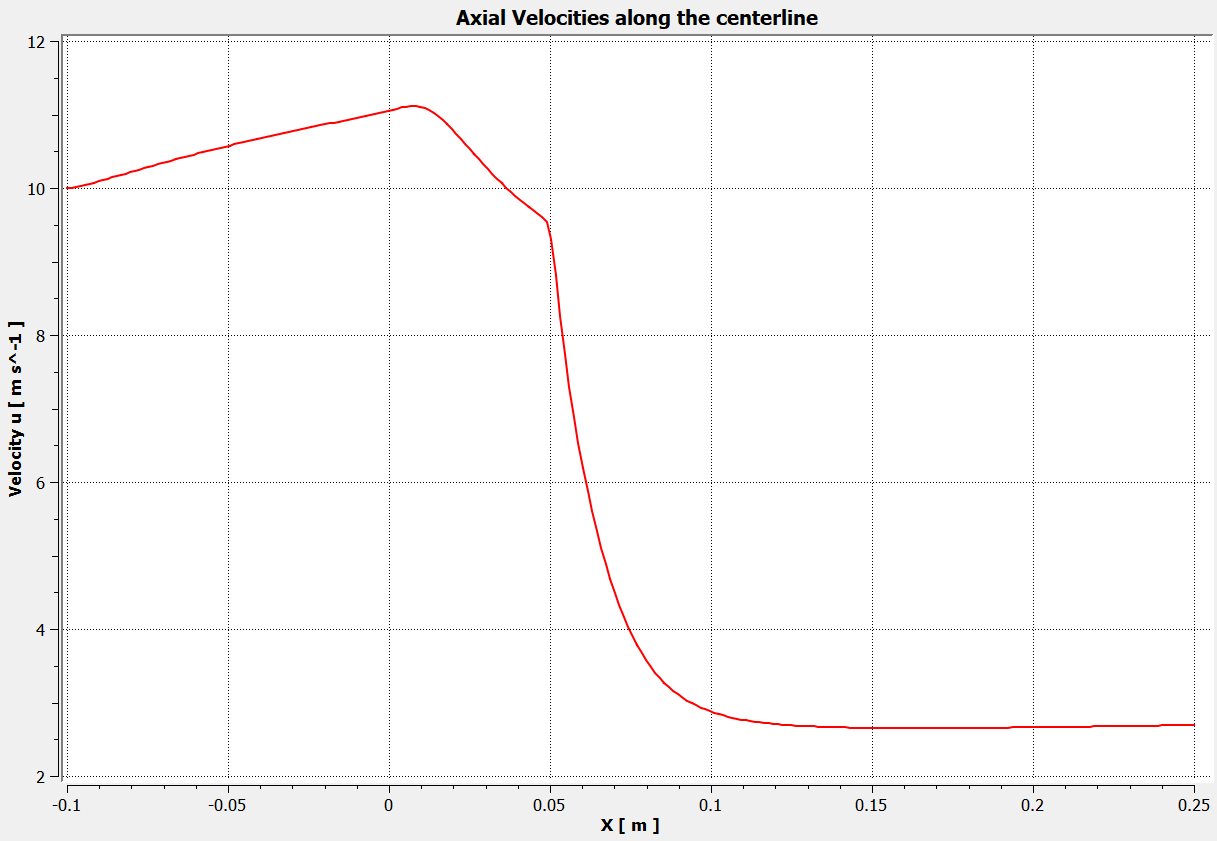
\includegraphics[width=.9\linewidth]{images/task2/task2-1/axial.png}
    \caption{Axial velocity profile of $k-\epsilon$ model}
    \label{fig:task2mesh}
    \end{subfigure}
    ~
\begin{subfigure}{.45\textwidth}
    \centering
    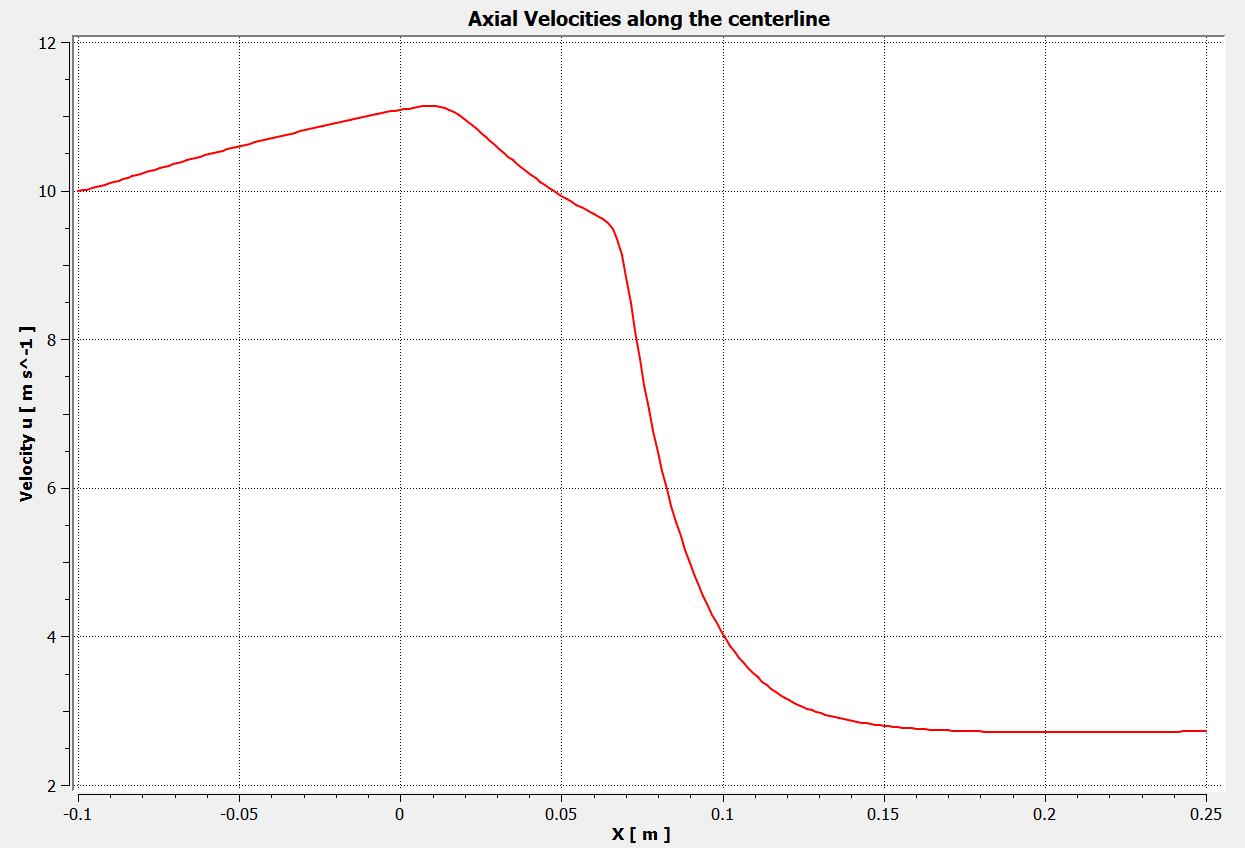
\includegraphics[width=.9\linewidth]{images/task2/task2-2/axials.png}
    \caption{Axial velocity profile of $k-\omega$ model}
    \label{fig:task2_residuals}
\end{subfigure}
    \caption{Axial velocity profiles}
    \label{fig:axial_task2}
\end{figure}


\noindent Further examination of the velocity profiles from different cross sections are shown comparatively on Figures \ref{fig:task2prof1} and \ref{fig:task2prof2}. On these plots, the discrepancies between the models are less apparent, especially in the vicinity of expansion. However, when looked at the cross sections from $x=20, 40, 60$ and $100 mm$ on Figure \ref{fig:task2prof2}, it can be clearly seen that the development of the boundary layer and the distribution of the axial velocities are different, especially near the walls of the pipe as expected since their behaviors near walls are what separates them mainly. \\


\noindent The profile for the $k-\omega$ model is closer to a parabolic shape than its alternative and shows a more realistic distribution of velocity. The $k-\epsilon$ model demonstrates irregular behavior with satisfying the no-slip condition by such rapid change in velocity near the wall. This is probably due to the inaccuracies seen in the damping functions near the walls. Specifically after 100mm, besides the steep decrease in velocity, the $k-\epsilon$ model shows a more uniform distribution of velocity throughout the cross section.



\begin{figure}[H]
    \centering
    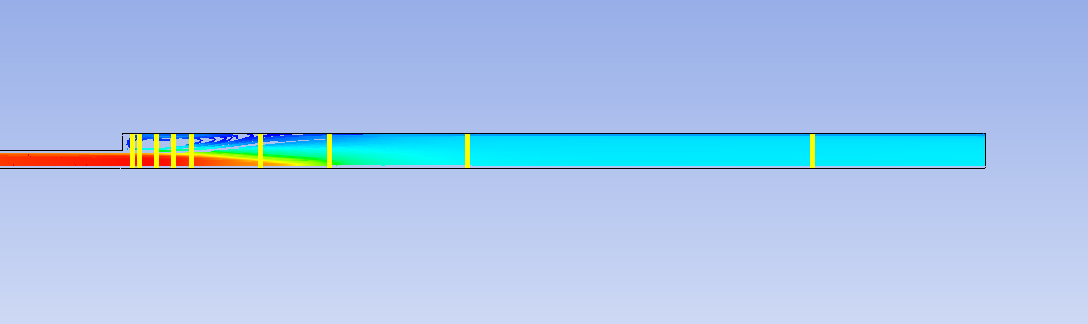
\includegraphics[width=.9\textwidth]{images/task2/task2-1/cross_section_locations.png}
    \caption{Cross Section Locations}
    \label{fig:task2cross}
\end{figure}


\begin{figure}[H]
    \centering
    \begin{subfigure}{.48\textwidth}
    \centering
    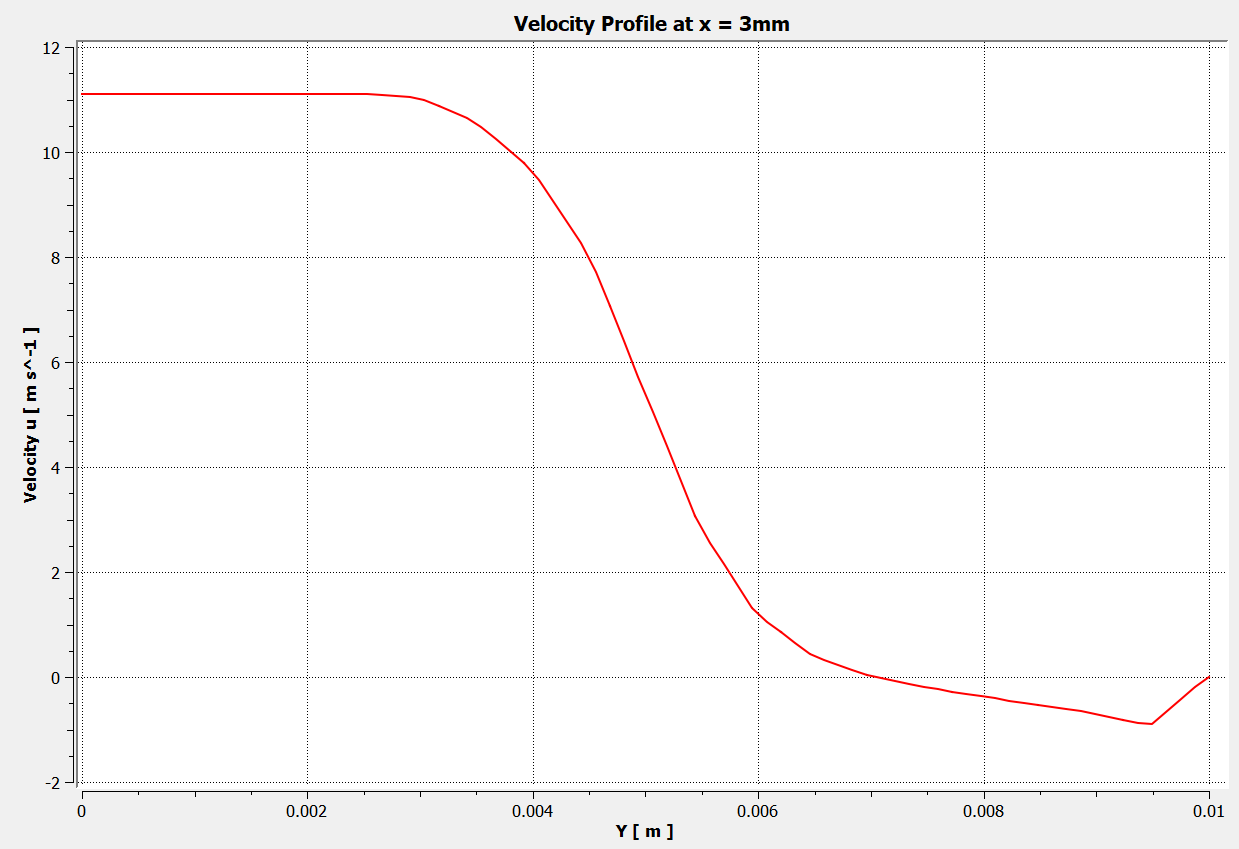
\includegraphics[width=.95\linewidth]{images/task2/task2-1/cs1.png}
    \caption{Velocity profile of $k-\epsilon$ model at x=3mm}
    \end{subfigure}
\hfill
\begin{subfigure}{.48\textwidth}
    \centering
    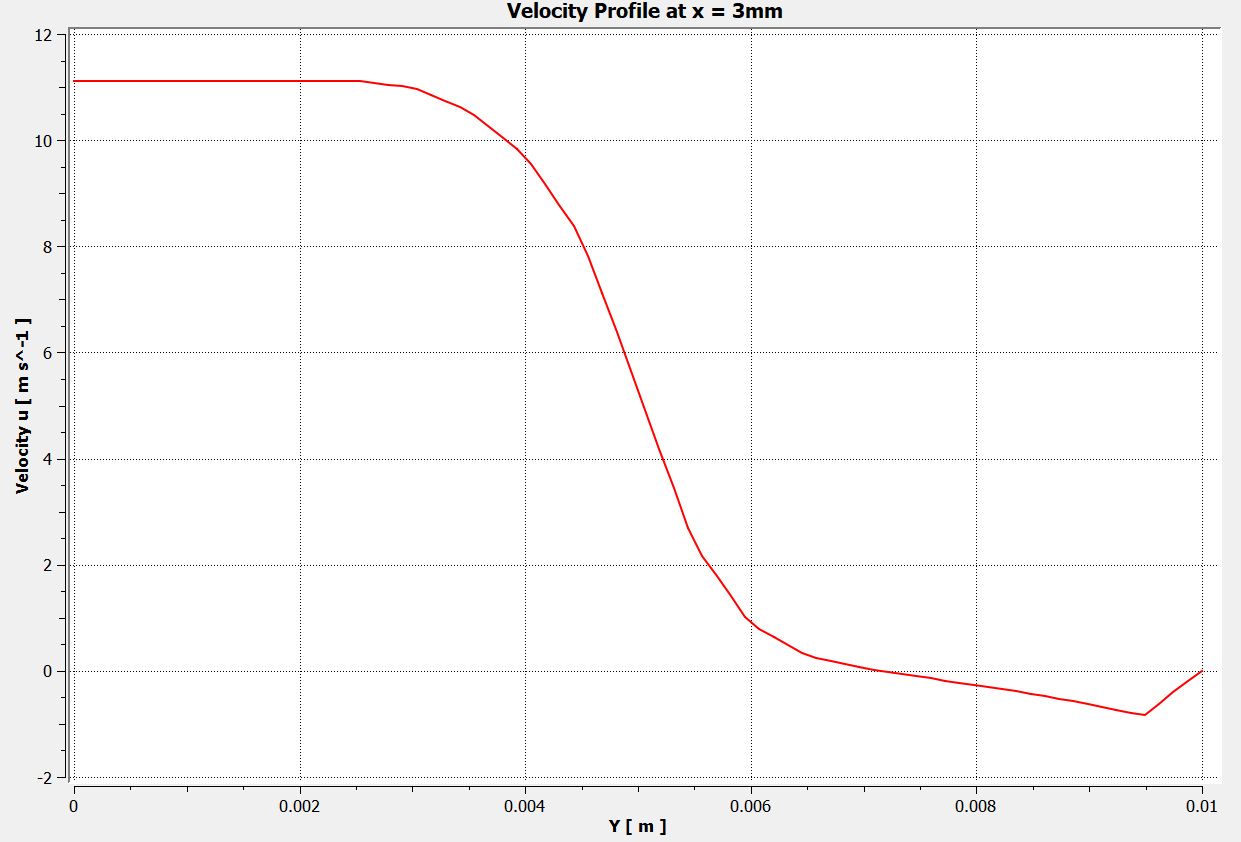
\includegraphics[width=.95\linewidth]{images/task2/task2-2/cs1.png}
    \caption{Velocity profile of $k-\omega$ model at x=3mm}
\end{subfigure}
    ~
    \begin{subfigure}{.48\textwidth}
    \centering
    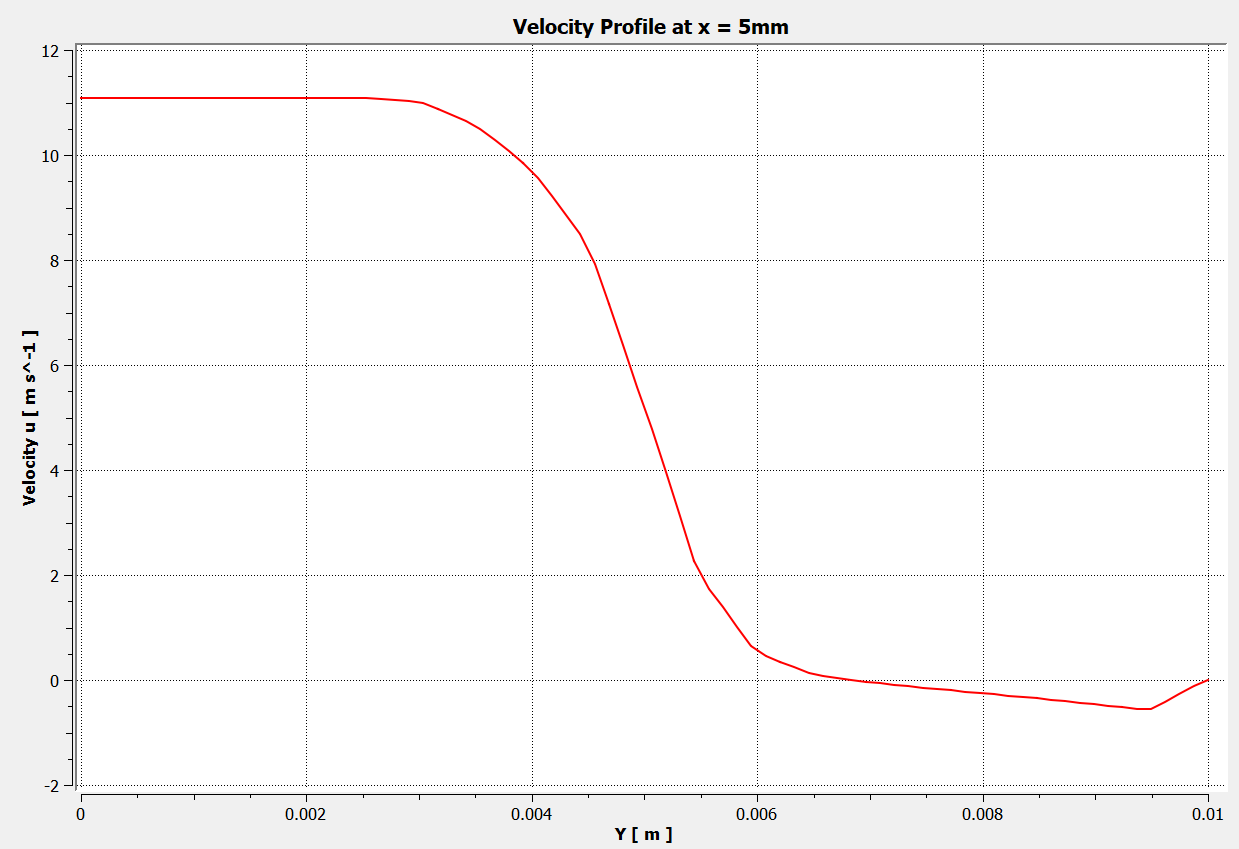
\includegraphics[width=.95\linewidth]{images/task2/task2-1/cs2.png}
    \caption{Velocity profile of $k-\epsilon$ model at x=5mm}
\end{subfigure}
    ~
    \begin{subfigure}{.48\textwidth}
    \centering
    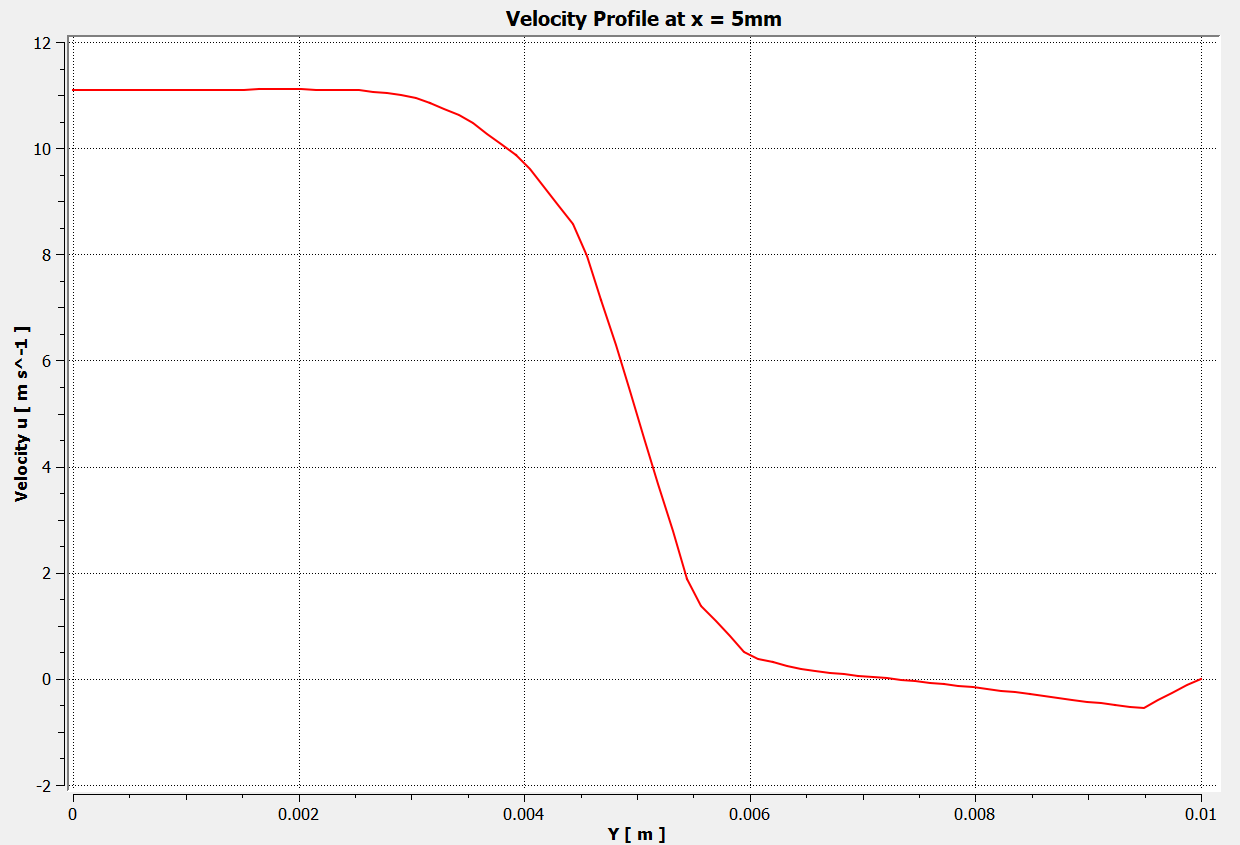
\includegraphics[width=.95\linewidth]{images/task2/task2-2/cs2.png}
    \caption{Velocity profile of $k-\omega$ model at x=5mm}
\end{subfigure}


    ~
    \begin{subfigure}{.48\textwidth}
    \centering
    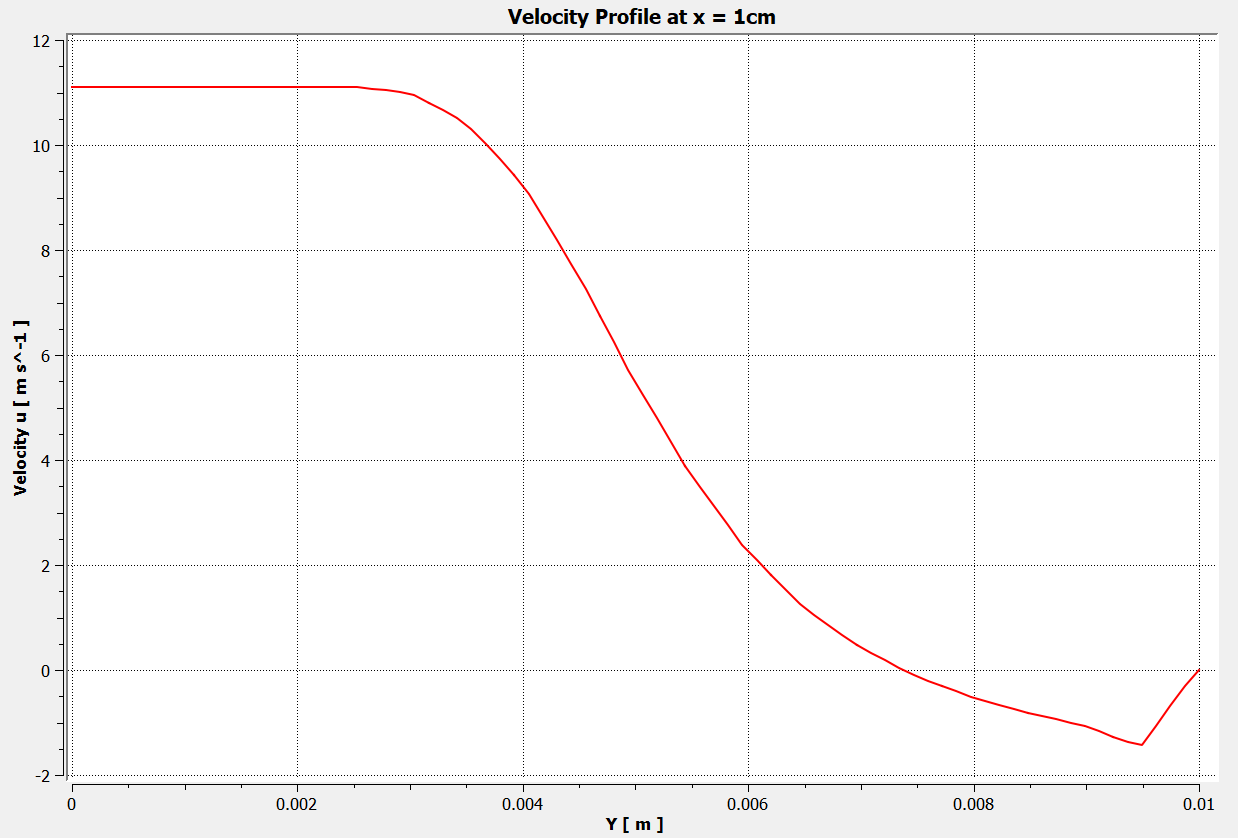
\includegraphics[width=.95\linewidth]{images/task2/task2-1/cs3.png}
    \caption{Velocity profile of $k-\epsilon$ model at x=10mm}
\end{subfigure}
    ~
    \begin{subfigure}{.48\textwidth}
    \centering
    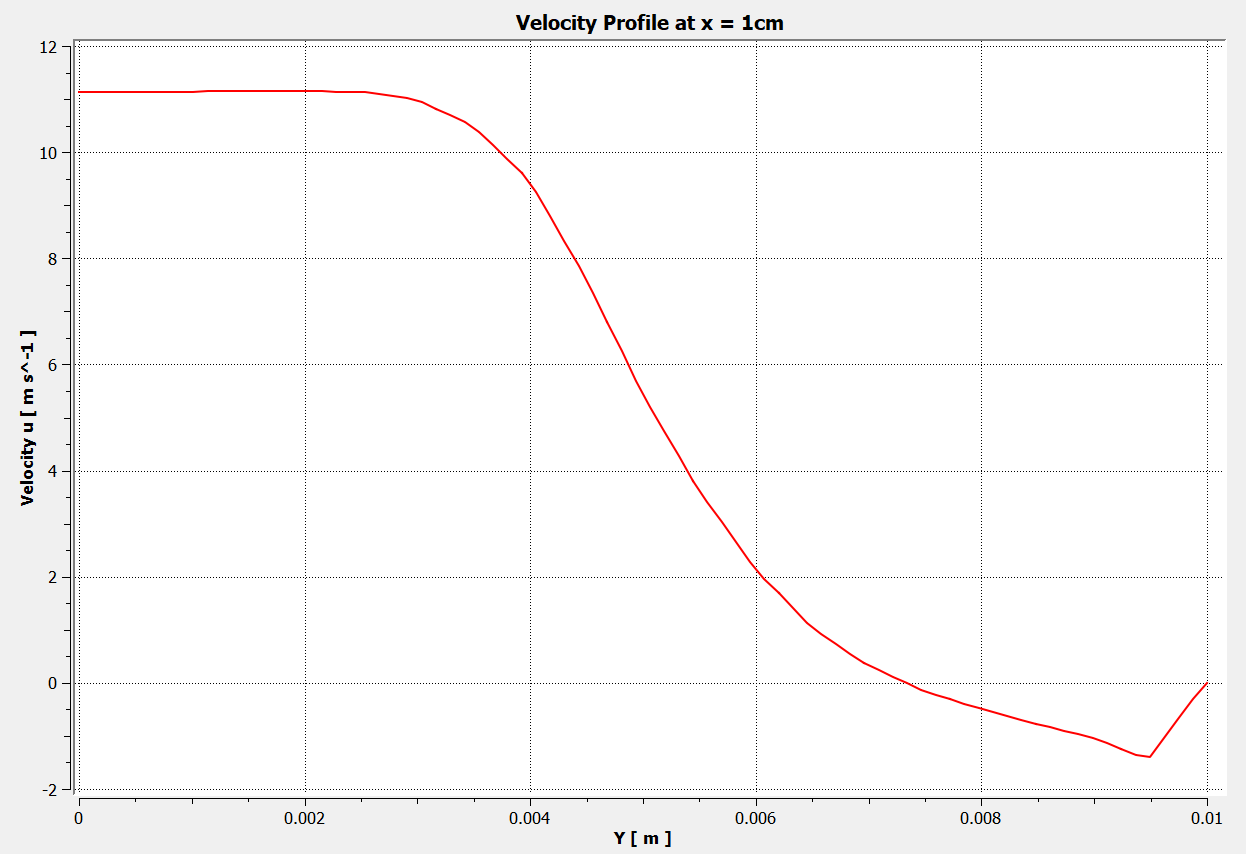
\includegraphics[width=.95\linewidth]{images/task2/task2-2/cs3.png}
    \caption{Velocity profile of $k-\omega$ model at x=10mm}
\end{subfigure}


    ~
    \begin{subfigure}{.48\textwidth}
    \centering
    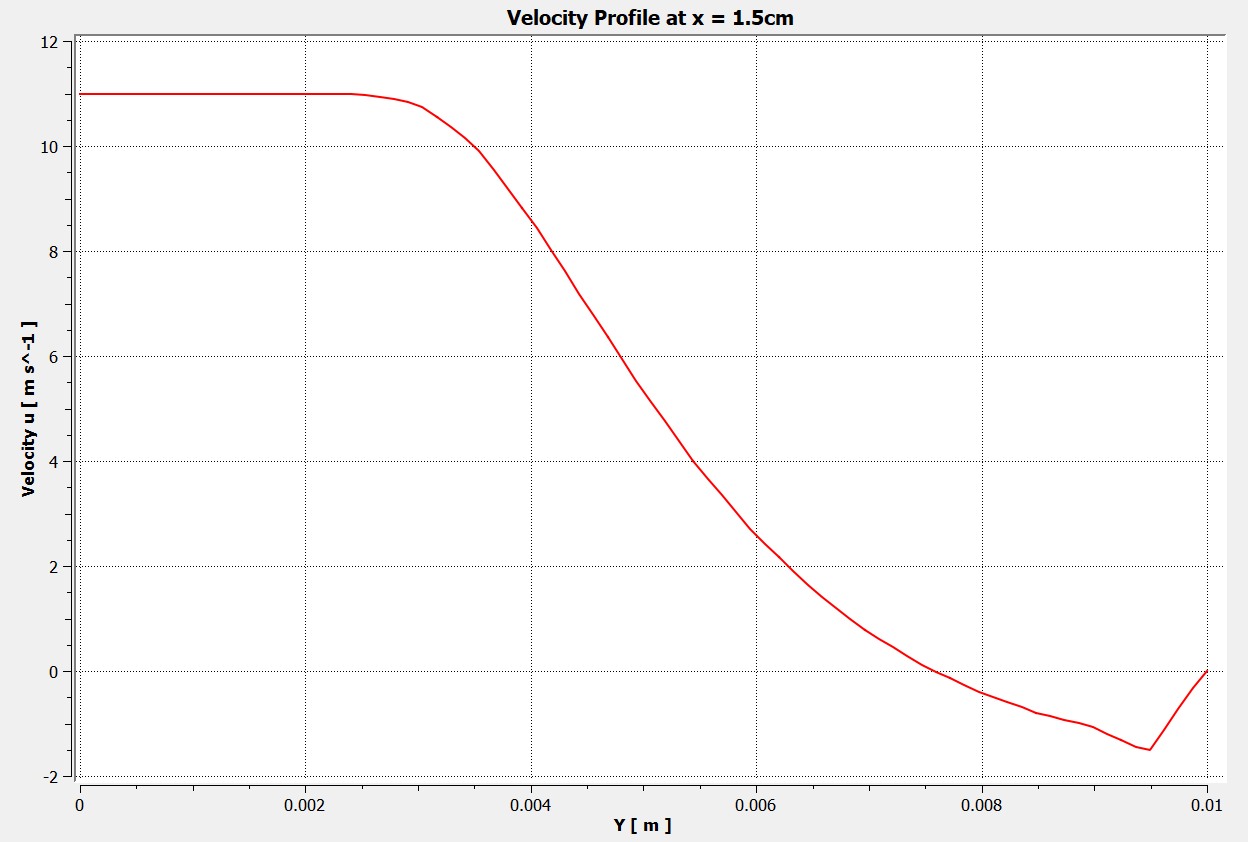
\includegraphics[width=.95\linewidth]{images/task2/task2-1/cs4.png}
    \caption{Velocity profile of $k-\epsilon$ model at x=15mm}
\end{subfigure}
    ~
    \begin{subfigure}{.48\textwidth}
    \centering
    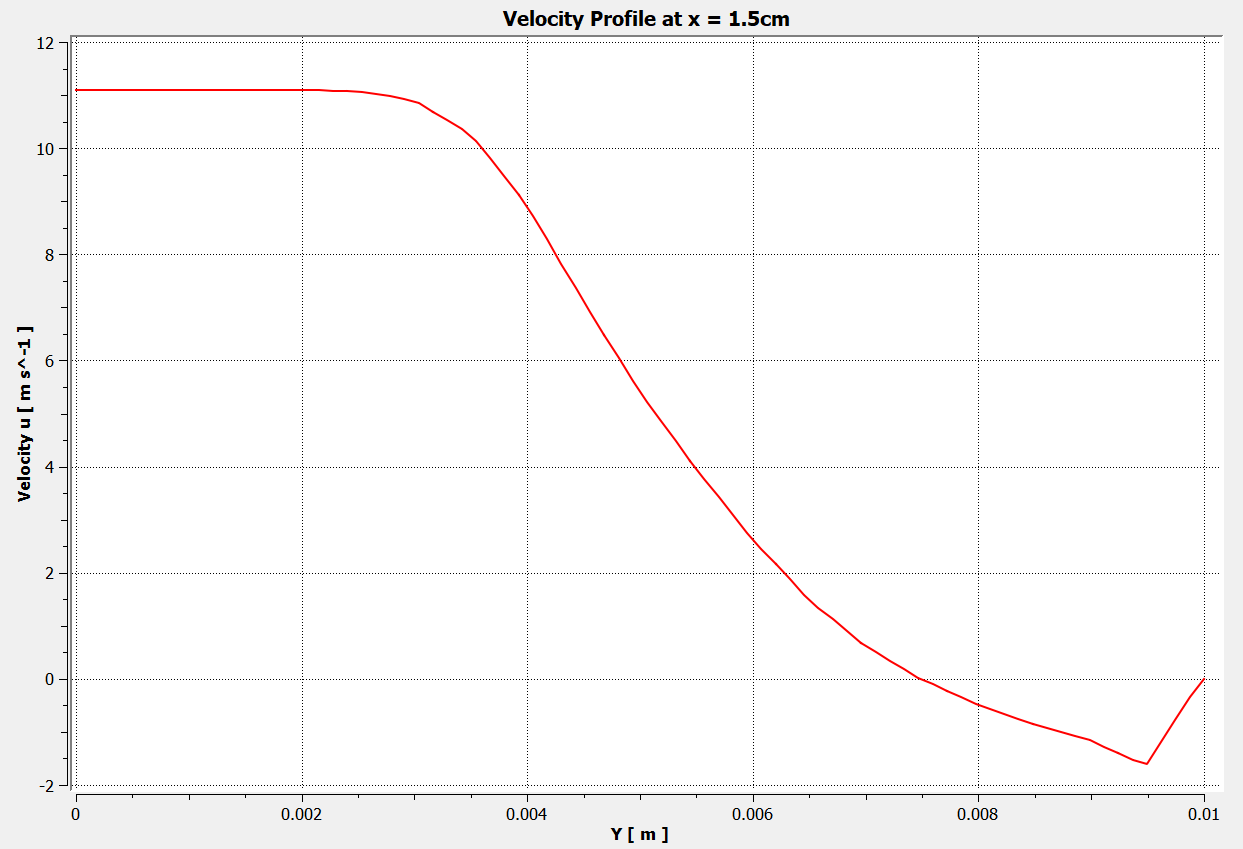
\includegraphics[width=.95\linewidth]{images/task2/task2-2/cs4.png}
    \caption{Velocity profile of $k-\omega$ model at x=15mm}
\end{subfigure}

    \caption{Velocity Profiles}
    \label{fig:task2prof1}
\end{figure}



\begin{figure}[H]
    \centering
     ~
    \begin{subfigure}{.48\textwidth}
    \centering
    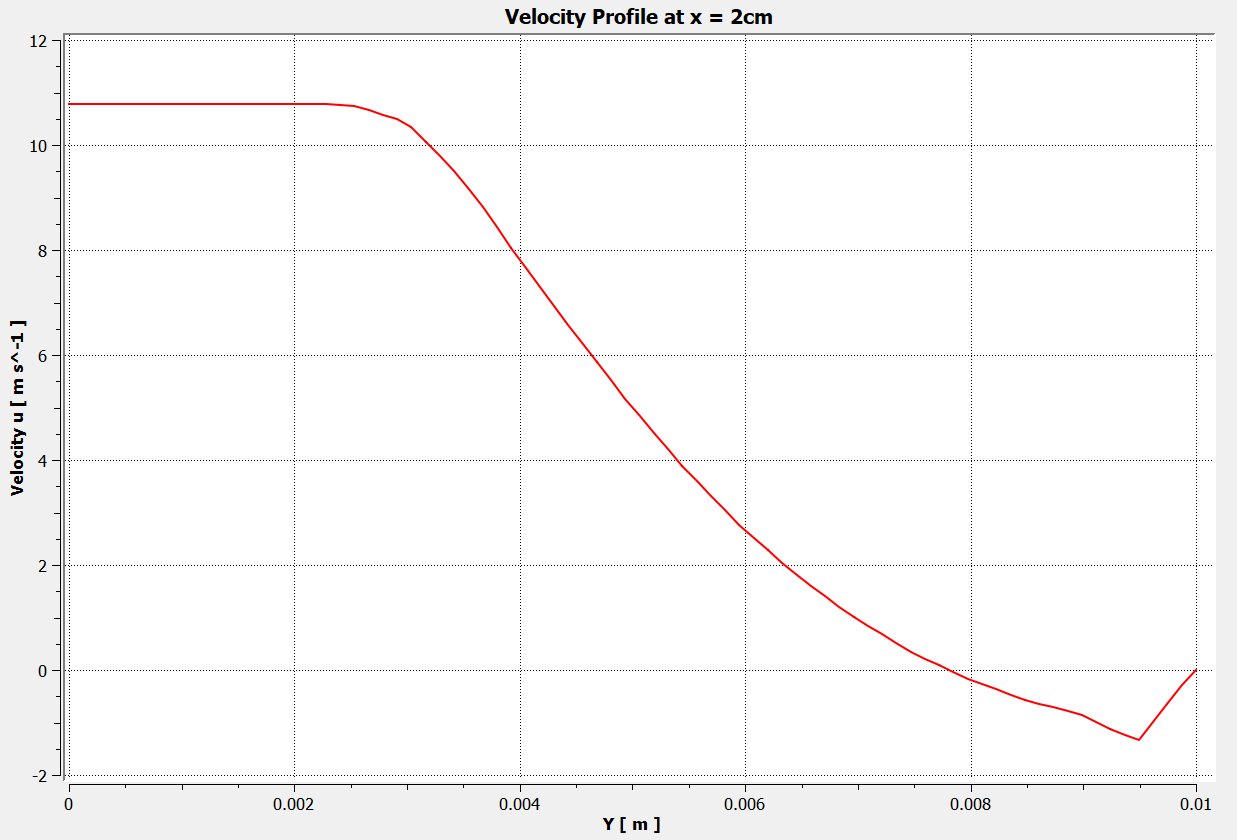
\includegraphics[width=.95\linewidth]{images/task2/task2-1/cs5.png}
    \caption{Velocity profile of $k-\epsilon$ model at x=20mm}
\end{subfigure}
    ~
    \begin{subfigure}{.48\textwidth}
    \centering
    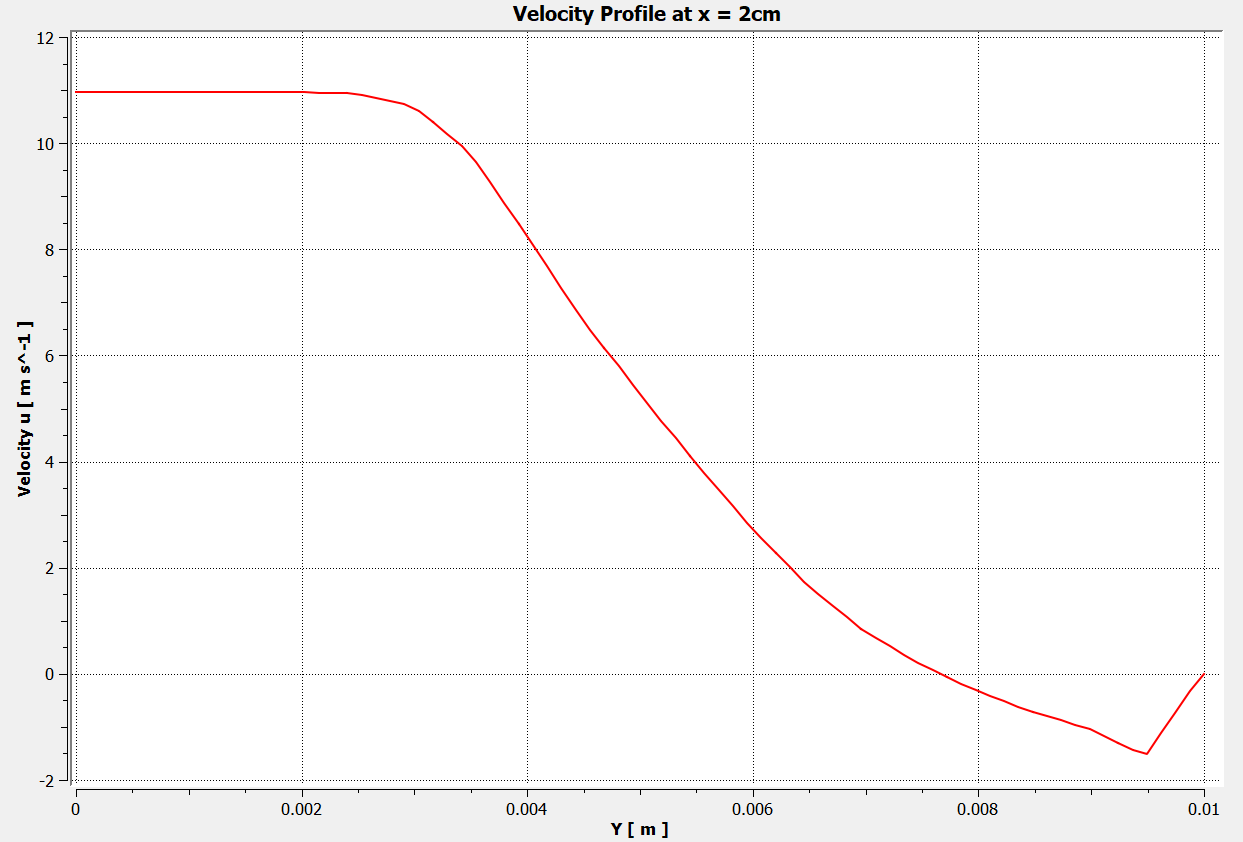
\includegraphics[width=.95\linewidth]{images/task2/task2-2/cs5.png}
    \caption{Velocity profile of $k-\omega$ model at x=20mm}
\end{subfigure}


     ~
    \begin{subfigure}{.48\textwidth}
    \centering
    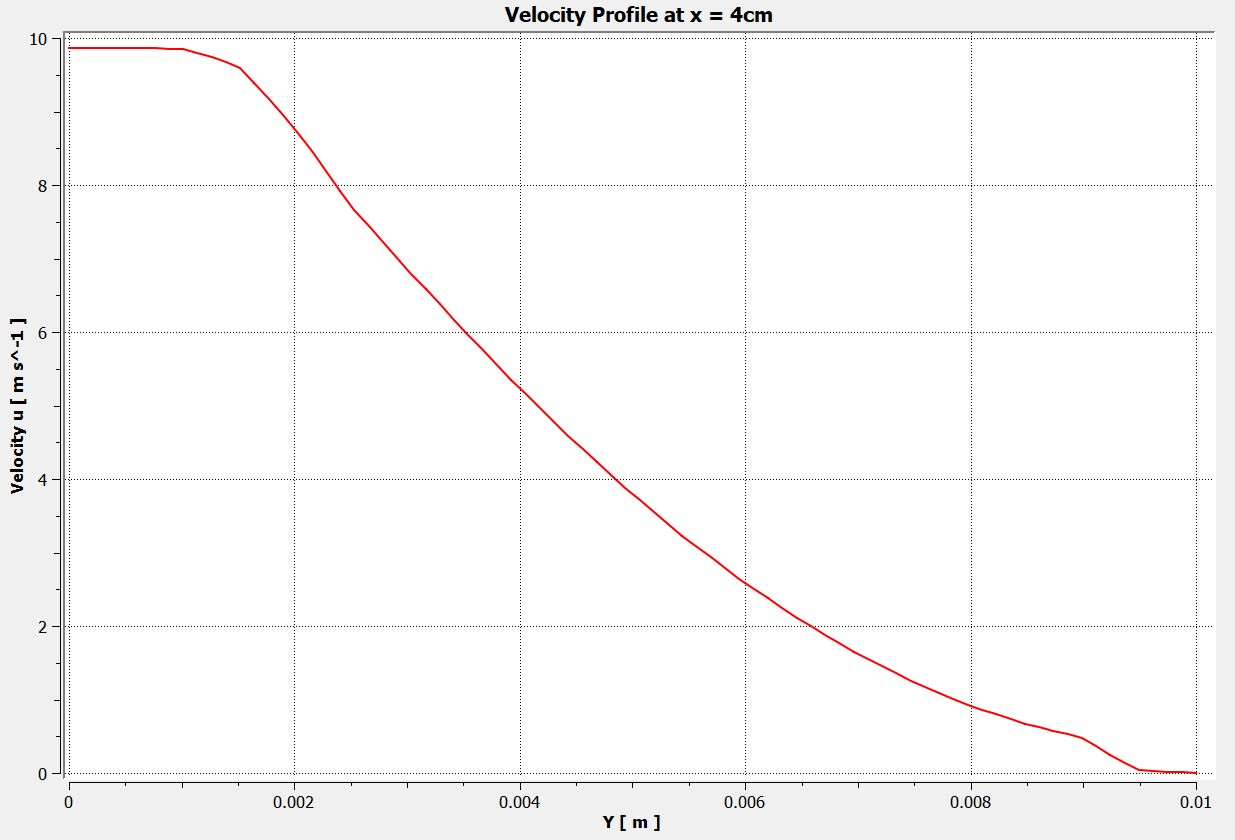
\includegraphics[width=.95\linewidth]{images/task2/task2-1/cs6.png}
    \caption{Velocity profile of $k-\epsilon$ model at x=40mm}
\end{subfigure}
    ~
    \begin{subfigure}{.48\textwidth}
    \centering
    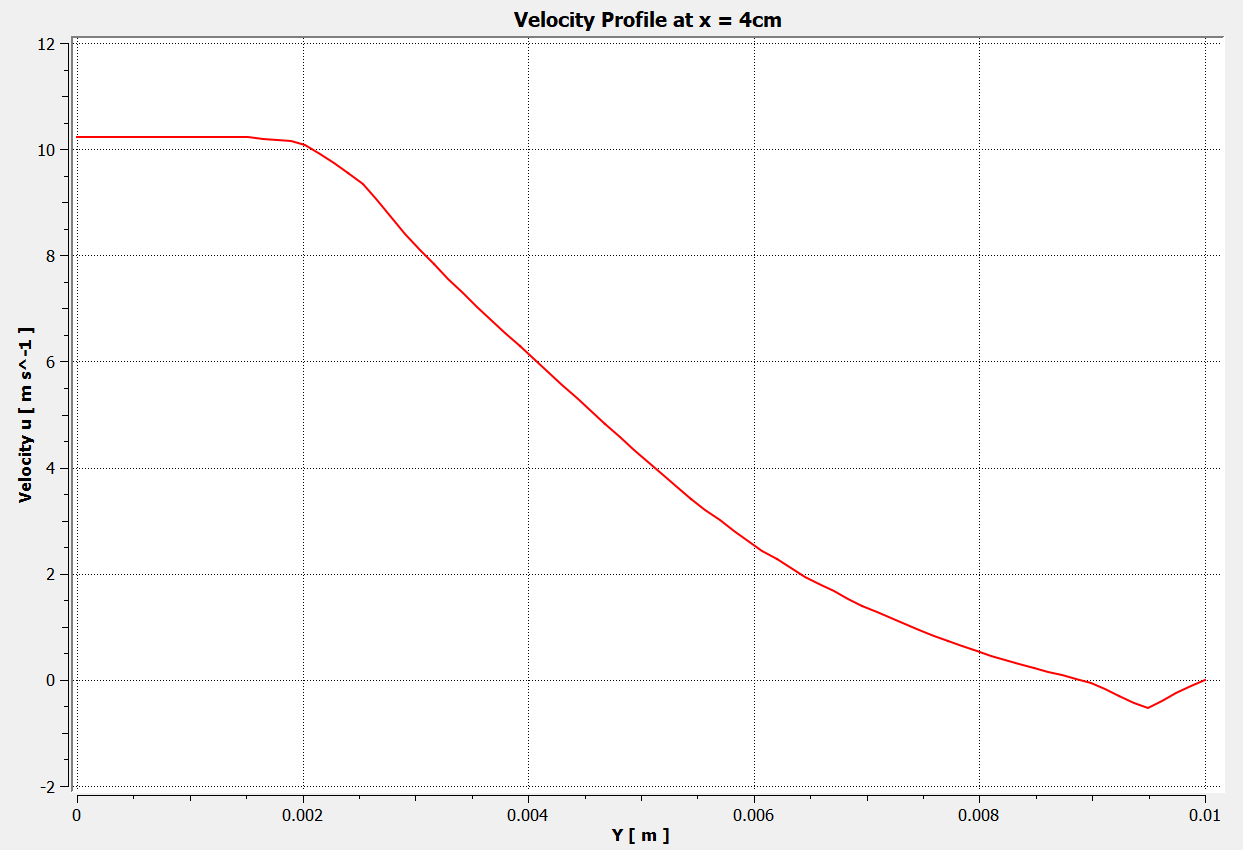
\includegraphics[width=.95\linewidth]{images/task2/task2-2/cs6.png}
    \caption{Velocity profile of $k-\omega$ model at x=40mm}
\end{subfigure}


     ~
    \begin{subfigure}{.48\textwidth}
    \centering
    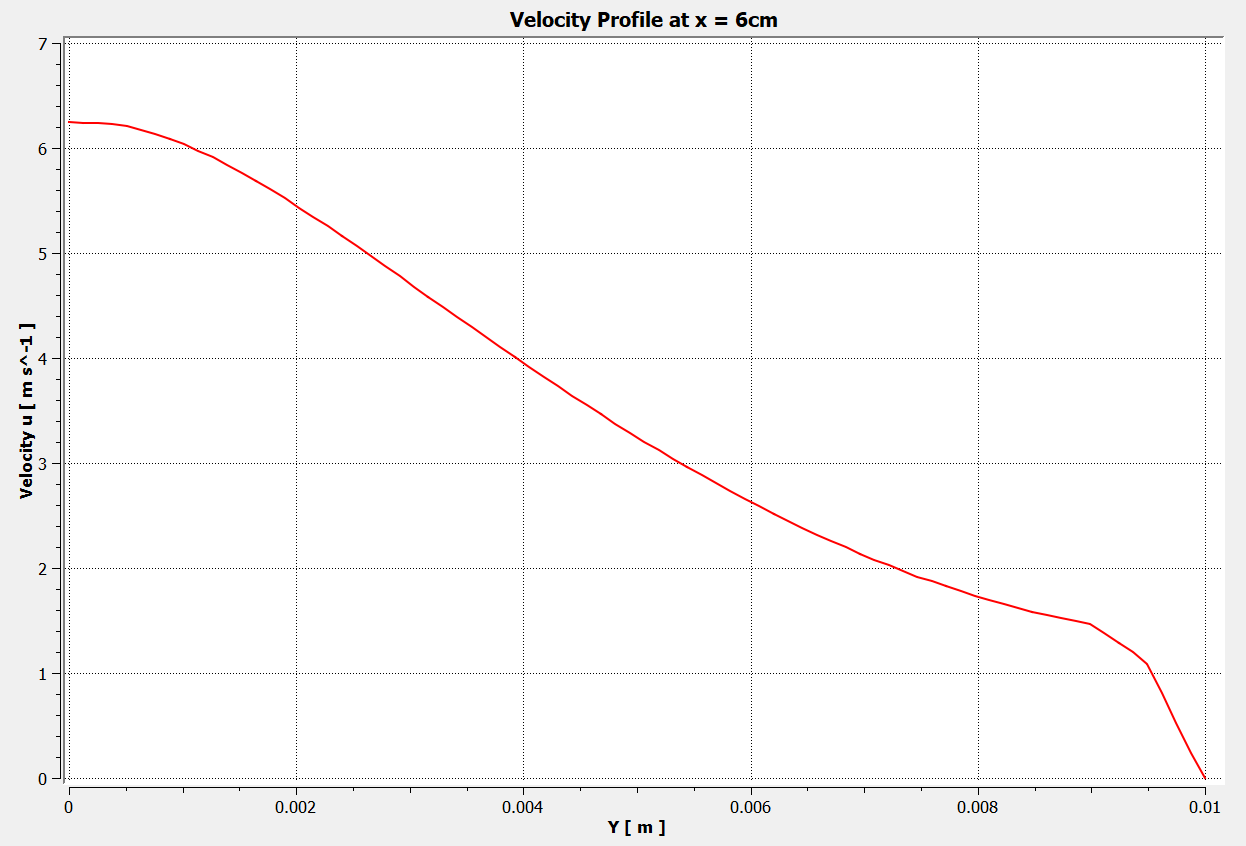
\includegraphics[width=.95\linewidth]{images/task2/task2-1/cs7.png}
    \caption{Velocity profile of $k-\epsilon$ model at x=4=60mm}
\end{subfigure}
    ~
    \begin{subfigure}{.48\textwidth}
    \centering
    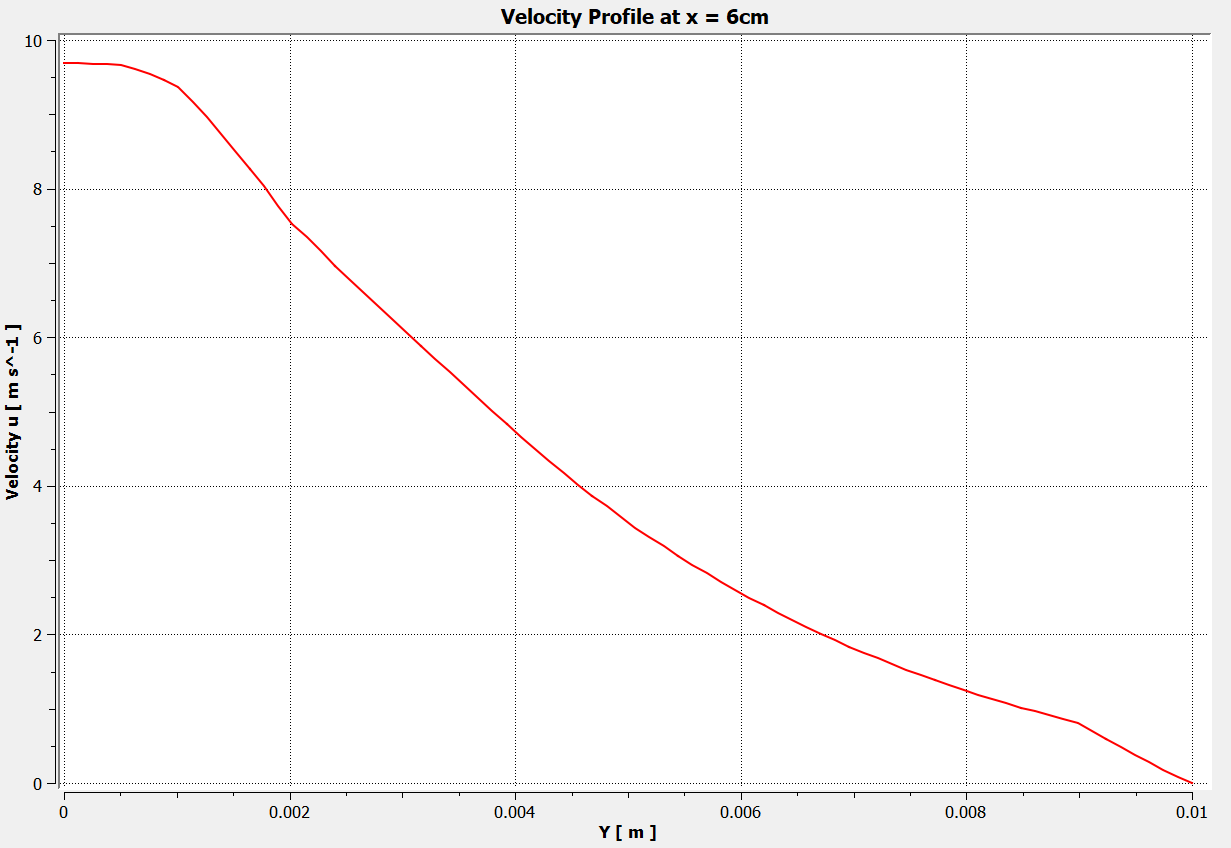
\includegraphics[width=.95\linewidth]{images/task2/task2-2/cs7.png}
    \caption{Velocity profile of $k-\omega$ model at x=4=60mm}
\end{subfigure}



     ~
    \begin{subfigure}{.48\textwidth}
    \centering
    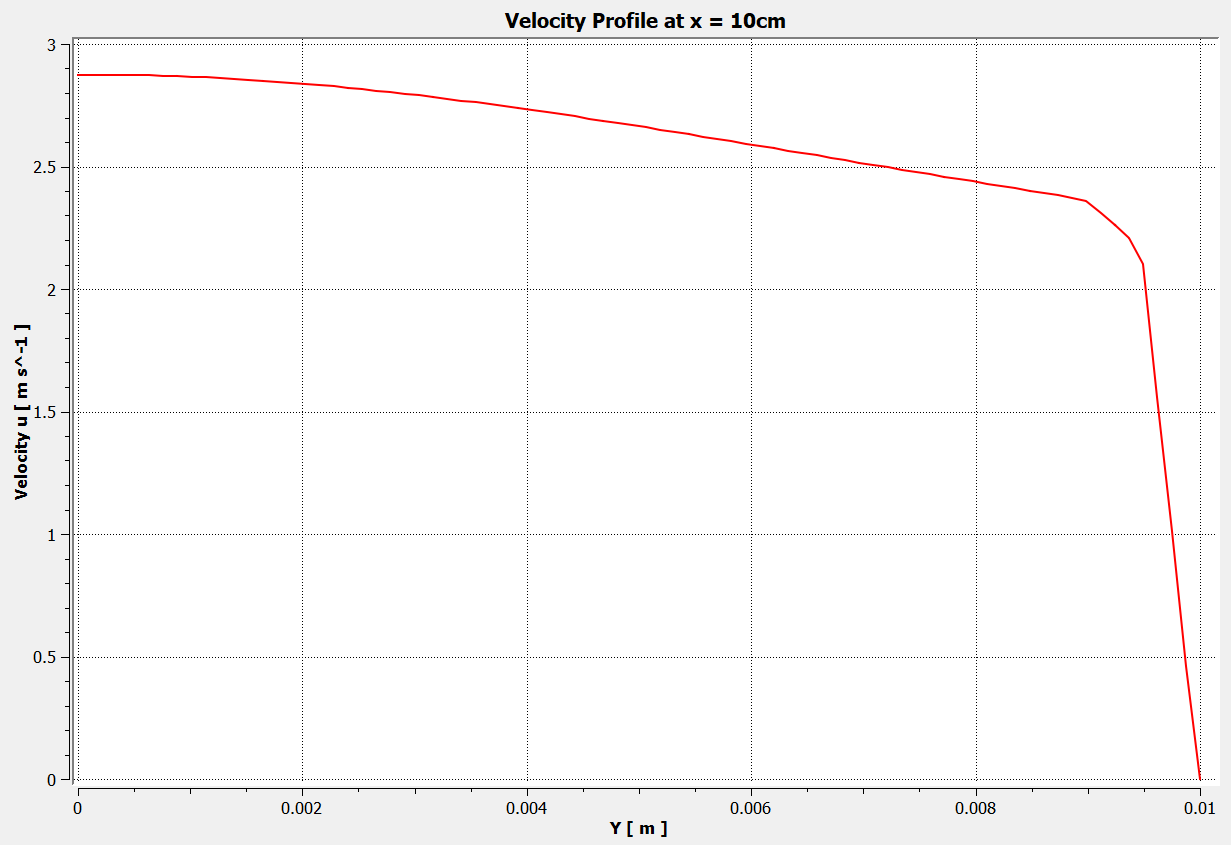
\includegraphics[width=.95\linewidth]{images/task2/task2-1/cs8.png}
    \caption{Velocity profile of $k-\epsilon$ model at x=100mm}
\end{subfigure}
    ~
    \begin{subfigure}{.48\textwidth}
    \centering
    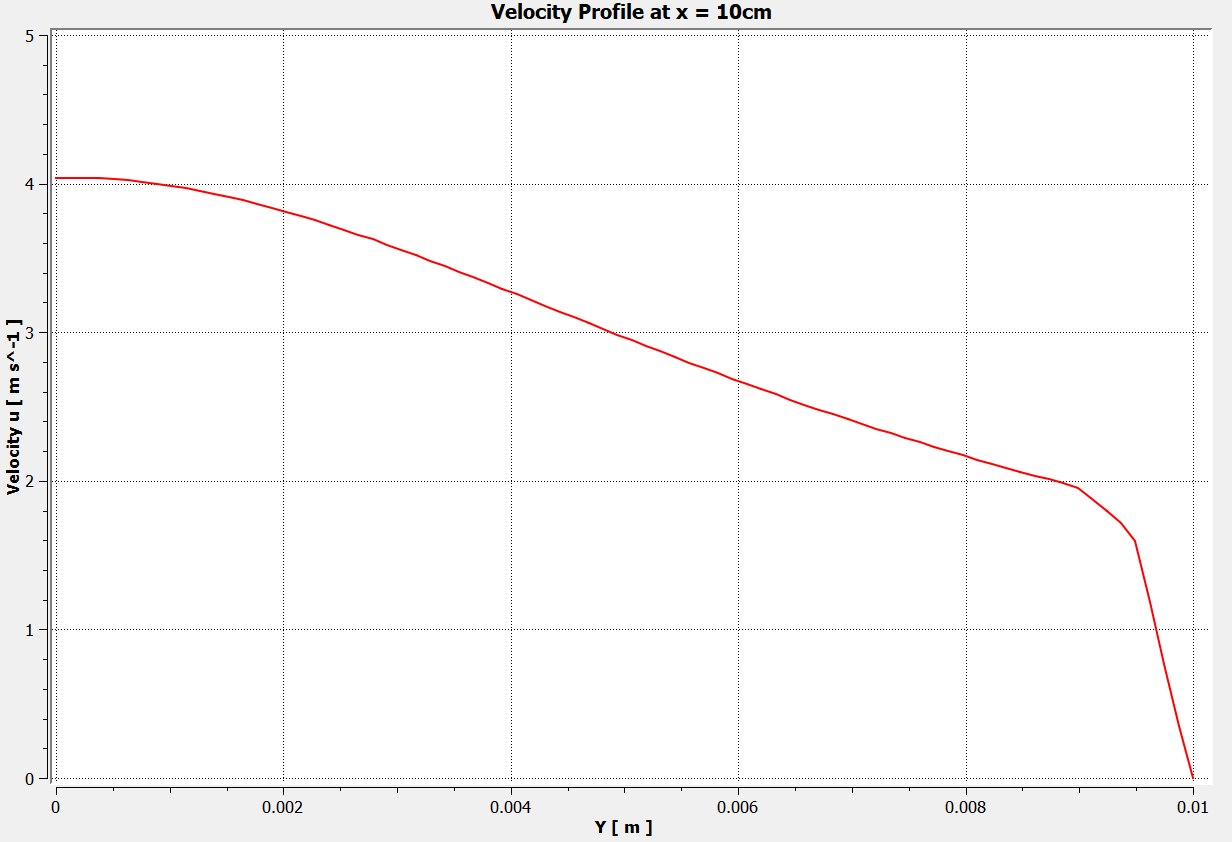
\includegraphics[width=.95\linewidth]{images/task2/task2-2/cs8.png}
    \caption{Velocity profile of $k-\omega$ model at x=100mm}
\end{subfigure}
    
    
    \caption{Velocity Profiles}
    \label{fig:task2prof2}
\end{figure}
\newpage

\subsubsection{Comparison of the Streamlines and Pressure Contours}

\noindent Now that we have seen velocity profiles, streamlines for the two models are the next to be examined. The figure below shows their comparison side-by-side. As guessed from their axial velocity profile, their recirculation zones are different in length. The $k-\omega$ model seems to result in a greater recirculation zone and a higher reattachment length. To support this, their reattachment lengths are shown on Table \ref{tab:task2}


\begin{figure}[H]
    \centering
    \begin{subfigure}{.8\textwidth}
    \centering
    \includegraphics[width=.8\linewidth]{images/task2/task2-1/2-1streamline.png}
    \caption{Streamlines of $k-\epsilon$ model}
    \end{subfigure}
    
\begin{subfigure}{.8\textwidth}
    \centering
    \includegraphics[width=.8\linewidth]{images/task2/task2-2/2-2streamline.png}
    \caption{Streamlines of $k-\omega$ model}
\end{subfigure}
    \caption{Streamlines}
    \label{fig:stream_task2}
\end{figure}


\begin{table}[H]
\centering
\caption{Reattachment Lengths of Models}
\begin{tabular}{c|c}
Model & Reattachment Length (m) \\ \hline
$k-\epsilon$  & 0.039                   \\
$k-\omega$   & 0.051                  
\end{tabular}

\label{tab:task2}
\end{table}

\noindent The last plot that will be of interest to us is the pressure contours in the vicinity of the recirculation zones. Those plots can be seen from Figure \ref{fig:press_task2}.

\begin{figure}[H]
    \centering
    \begin{subfigure}{.85\textwidth}
    \centering
    \includegraphics[width=.9\linewidth]{images/task2/task2-1/2-1pressure.png}
    \caption{Pressure contours of $k-\epsilon$ model}
    \end{subfigure}
    
\begin{subfigure}{.85\textwidth}
    \centering
    \includegraphics[width=.9\linewidth]{images/task2/task2-2/2-2pressure.png}
    \caption{Pressure contours of $k-\omega$ model}
\end{subfigure}
    \caption{Pressure Contours}
    \label{fig:press_task2}
\end{figure}


\noindent As expected there is a pressure drop induced by the expansion of the pipes. Similar to the streamlines and velocity profiles, the zone in which the pressure drops the most is wider in the $k-\omega$ model, which is in agreement with all the other deductions we have made up to this point. Again caused by turbulences and vortices we observe, the pressure drop return back to normal after some distance from the expansion.

\subsection{Task 3}

As described in Section \ref{sec:task3intro}, several different cases of expansion have been studied and processed. For each case, streamlines have been plotted and pressure contours have been drawn. As expected, there is a drop in pressure after the fluid goes through the expansion. \\

\noindent Geometries and flows with different expansion ratios and their results are shown below. In each variation of the simulation, grid convergence have been checked to ensure meaningful results and interpretations. The converged element size was found at $10^{-3}$ meters. Also, residual parameters are verified to have reduced under tolerated values and the input and output fluxes are checked and verified to have the same magnitude (difference in fluxes are in the order of $10^{-9}$).\\

\noindent To compare the pressure differences using the equations \ref{eq:hm} and \ref{eq:headlosscoeff}, we can combine them and obtain the following formula which yields pressure difference from average velocity, density and K.

\begin{equation}
    \Delta p = \frac{K * V^2 * \rho}{2}
    \label{eq:final_dP}
\end{equation}

\subsubsection{Sudden and Moderate Expansion ($\frac{d}{D} = 0.6$)}

Using equation \ref{eq:final_dP}, the expected theoretical pressure drop can be calculated when K value is found from Figure \ref{fig:exp_plots} to be 0.4:

\[\Delta p = \frac{0.4 * 0.554^2 * 100}{2} = 6.138Pa \]


\noindent The red circles on Figure \ref{fig:06_locs} shows the locations of the probes used to take samples of pressures before and after the expansion. The value from the probe before the expansion is taken to be 32.7 Pa, while it is observed to have dropped to 26.1 Pa. This results in a $\Delta p$ of 6.6 Pa, which is \textbf{within 7.5\% error} of what is expected.

\begin{figure}[H]
    \centering
    \includegraphics[width=.7\linewidth]{images/task3/06_locations.png}
    \caption{Pressure drop probe locations for moderate expansion}
    \label{fig:06_locs}
\end{figure}


\subsubsection{Sudden and Significant Expansion ($\frac{d}{D} = 0.4$)}

Using equation \ref{eq:final_dP}, the expected theoretical pressure drop can be calculated when K value is found from Figure \ref{fig:exp_plots} to be 0.7:

\[\Delta p = \frac{0.7 * 0.554^2 * 100}{2} = 10.74Pa \]


\noindent The red circles on Figure \ref{fig:04_locs} shows the locations of the probes used to take samples of pressures before and after the expansion. The value from the probe before the expansion is taken to be 20.2 Pa, while it is observed to have dropped to 8.9 Pa. This results in a $\Delta p$ of 6.6 Pa, which is \textbf{within 5.2\% error} of what is expected. Also, the streamlines for this case can be seen in Figure \ref{fig:04_stream}.

\begin{figure}[H]
\centering
\hfill
\begin{subfigure}{.48\textwidth}
    \includegraphics[width=.95\linewidth]{images/task3/04_locations.png}
    \caption{Pressure drop probe locations for significant expansion}
    \label{fig:04_locs}
\end{subfigure}
\hfill
\begin{subfigure}{.48\textwidth}
    \includegraphics[width=.95\linewidth]{images/task3/04_streamlines.png}
    \caption{Streamlines for significant expansion}
    \label{fig:04_stream}
\end{subfigure}
\label{fig:04_figure}
\caption{Significant expansion pressure and streamlines}
\end{figure}


\subsubsection{Sudden and Severe Expansion ($\frac{d}{D} = 0.2$)}

Using equation \ref{eq:final_dP}, the expected theoretical pressure drop can be calculated when K value is found from Figure \ref{fig:exp_plots} to be 0.91:

\[\Delta p = \frac{0.91 * 0.554^2 * 100}{2} = 13.96Pa \]


\noindent The red circles on Figure \ref{fig:02_locs} shows the locations of the probes used to take samples of pressures before and after the expansion. The value from the probe before the expansion is taken to be 16.2 Pa, while it is observed to have dropped to 3.5 Pa. This results in a $\Delta p$ of 12.7 Pa, which is \textbf{within 9\% error} of what is expected. Also, the streamlines for this case can be seen in Figure \ref{fig:02_stream}.


\begin{figure}[H]
\centering
\hfill
\begin{subfigure}{.48\textwidth}
    \includegraphics[width=.95\linewidth]{images/task3/02_locations.png}
    \caption{Pressure drop probe locations for severe expansion}
    \label{fig:02_locs}
\end{subfigure}
\hfill
\begin{subfigure}{.48\textwidth}
    \includegraphics[width=.95\linewidth]{images/task3/02_streamlines.png}
    \caption{Streamlines for severe expansion}
    \label{fig:02_stream}
\end{subfigure}
\label{fig:02_figure}
\caption{Severe expansion pressure and streamlines}
\end{figure}


\subsubsection{Gradual and Moderate Expansion ($\frac{d}{D} = 0.4$)}

Using equation \ref{eq:final_dP}, the expected theoretical pressure drop can be calculated when K value is found from Figure \ref{fig:exp_plots} to be 0.91 (However, this time the plot for gradual expansion at a cone angle of $20^{\circ}$ is used):

\[\Delta p = \frac{0.38 * 0.554^2 * 100}{2} = 5.83Pa \]


\noindent The red circles on Figure \ref{fig:04_gradual_locs} shows the locations of the probes used to take samples of pressures before and after the expansion. The value from the probe before the expansion is taken to be 20.1 Pa, while it is observed to have dropped to 13.4 Pa. This results in a $\Delta p$ of 6.7 Pa, which is \textbf{within 13\% error} of what is expected. Also, the streamlines for this case can be seen in Figure \ref{fig:04_gradual_stream}. When examined, it can be clearly said that the gradual expansion did not induce a recirculation zone as it was observed for all sudden expansion cases, including tasks 1 and 2. Also, it causes less pressure drop when compared with sudden expansion for the same expansion ratio. The loss in pressure is lower in this case due to more laminar-like and less turbulent nature of the fluid inside the gradual expansion. The lack of recirculations affect the behavior and the properties of the fluid dearly.

\begin{figure}[H]
\centering

\begin{subfigure}{.48\textwidth}
    \includegraphics[width=.95\linewidth]{images/task3/04_gradual_locations.png}
    \caption{Pressure drop probe locations for gradual expansion}
    \label{fig:04_gradual_locs}
\end{subfigure}
\hfill
\begin{subfigure}{.48\textwidth}
    \includegraphics[width=.95\linewidth]{images/task3/04_gradual_press.png}
    \caption{Pressures for gradual expansion}
    \label{fig:04_gradual_pressure}
\end{subfigure}

\begin{subfigure}{.8\textwidth}
    \includegraphics[width=.95\linewidth]{images/task3/04_gradual_streamlines.png}
    \caption{Streamlines for gradual expansion}
    \label{fig:04_gradual_stream}
\end{subfigure}

\label{fig:gradual_figure}
\caption{Gradual expansion pressure and streamlines and locations}
\end{figure}


\subsubsection{Optimization of the Expansion for $\frac{d}{D} = 0.5$}

As introduced in section \ref{sec:task3intro}, two different cases for expansion are studied. Among these two, for an expansion ratio of $0.5$, we have two options to choose, a sudden or a gradual expansion. The simulations and comparisons, along with equation \ref{eq:final_dP}, show that the smaller the K constant, the less pressure drop occurs. As can be seen from Figure \ref{fig:cone_angle}, the smallest K number that corresponds to 0.5 expansion ratio is found at a gradual expansion of around $7.6^{\circ}$. \\

\noindent Using those values, minimum K in estimated to be 2.5 which is shown in Figure \ref{fig:cone_angle}. Using that K value, the estimated pressure loss becomes:
\[\Delta p = \frac{0.25 * 0.554^2 * 100}{2} = 3.84Pa \]


\begin{figure}[H]
    \centering
    \includegraphics[width=.6\linewidth]{images/task3/cone_angle.png}
    \caption{Smallest K for a gradual expansion with a ratio of 0.5 \cite{white_chul_2016}}
    \label{fig:cone_angle}
\end{figure}


\noindent This 3.84Pa drop is the lowest observed during all previous expansion cases. Furthermore, according to the plot given by White's book, it is the lowest drop possible for 0.5 expansion ratio. The geometry has been modified to have a gradual expansion of said angle and the simulation has been run accordingly. The residuals, steady state conditions and grid convergence has been verified. The mesh independent results are plotted and can be seen from Figure \ref{fig:opt_figure}. 


\begin{figure}[H]
\centering

\begin{subfigure}{.48\textwidth}
    \includegraphics[width=.95\linewidth]{images/task3/optimized_locations.png}
    \caption{Pressure drop probe locations for optimized expansion}
    \label{fig:04_gradual_locs}
\end{subfigure}
\hfill
\begin{subfigure}{.48\textwidth}
    \includegraphics[width=.95\linewidth]{images/task3/optimized_pressure.png}
    \caption{Pressures for optimized expansion}
    \label{fig:04_gradual_pressure}
\end{subfigure}

\begin{subfigure}{.7\textwidth}
    \includegraphics[width=.95\linewidth]{images/task3/optimized_streamline.png}
    \caption{Streamlines for optimized expansion}
    \label{fig:04_gradual_stream}
\end{subfigure}

\caption{Optimized expansion pressure and streamlines and locations}
\label{fig:opt_figure}
\end{figure}



\noindent To sum up, it can be said that with the data we have in our disposal, \textbf{a gradual expansion with a cone angle of 7.6 degrees} is the optimum setup for minimum pressure loss caused by the expansion.



%%%%%%%%%%%%%%%%%%%% Conclusion %%%%%%%%%%%%%%%%%%%%%
\section{Conclusion}

In this report many different properties and behaviors of fluid flow through an expansion is studied. The flow is simulated for both laminar and turbulent behavior and different expansion ratios and types are analyzed and interpreted. Lastly, an optimized neck for the expansion has been found and tested.\\

\noindent It has been observed that due to turbulent mixing seen in the vicinity of the expansion, these is a loss in the mechanical energy of the fluid which causes a pressure drop on the fluid. This drop has been modeled mathematically and our simulations seemed to be in almost fully agreement with the theoretical values for both pressure drops and velocity profiles.\\

\noindent Furthermore, other properties like the reattachment length of the recirculation zone has been interpreted and there was found a good correlation between our simulation results and experimental results taken from the study of Hammad et al.\cite{hammad_ötügen_arik_1999}. It was surprising how close our results were to both theoretical and experimental data available. \\

\noindent This project was surely a head-first introduction to Computational Fluid Dynamics for me as it was the first time I used these functionalities of ANSYS. While challenging, it was an exciting and fruitful endeavor for me.

\printbibliography
\end{document}